\documentclass[a4paper, 11pt]{article}
 


%%%%%%%%%%%%%%%%%%%%%%%%%%%%%%%%%
%	 PACKAGES	%
%%%%%%%%%%%%%%%%%%%%%%%%%%%%%%%%%
% Codierung von in und Output
\usepackage[utf8]{inputenc}
\usepackage[T1]{fontenc}

% AMS-Pakete für Mathe
\usepackage{amsthm,amssymb,amsmath}
\usepackage{cancel} %Durchgestrichene Symbole

% Sprachpaket neue rechtschreibung
\usepackage[ngerman]{babel}


\usepackage[most]{tcolorbox}

%Header und Seitengrösse
\usepackage{fancyhdr}
\usepackage{geometry}

% Paket für Links im PDF (glaubs)!
\usepackage[hidelinks]{hyperref}

%Paket um ganze pdf-File zu importieren (Arbeitsblätter aus Analysis DMK)
\usepackage{pdfpages}

%TColorbox nutzt Theoreme und bessere Verweise
\tcbuselibrary{theorems}
\usepackage{cleveref}
\crefname{section}{Kapitel}{Kapitel}
\Crefname{section}{Kapitel}{Kapitel}

%Package, um Aufgaben auf mehrere Spalten zu verteilen.
\usepackage{tasks}

%Tikz
\usepackage{tikz}
\usepackage{pgfplots}
\pgfplotsset{compat=1.18}




%Programmcode-Darstellung
\usepackage{listings}
\usepackage{xcolor}
\lstset{basicstyle=\ttfamily}
\definecolor{codekeyword}{rgb}{0.11,0.53,0.63}
\definecolor{codenumbers}{rgb}{0.71,0.21,0.30}
\definecolor{codeoperation}{rgb}{0.57,0.32,0.59}
\definecolor{codecomment}{rgb}{0.17,0.59,0.28}
\definecolor{backcolour}{rgb}{0.98,0.97,0.99}
\definecolor{codestring}{rgb}{0.84,0.56,0.16}
\lstdefinestyle{mystyle}{
	backgroundcolor=\color{backcolour},
	commentstyle=\color{codecomment},
	keywordstyle=\color{codekeyword},
	numberstyle=\tiny\color{black},
	stringstyle=\color{codestring},
	basicstyle=\ttfamily\footnotesize,
	breakatwhitespace=false,
	breaklines=true,
	captionpos=b,
	keepspaces=true,
	numbers=left,
	numbersep=5pt,
	showspaces=false,
	showstringspaces=false,
	showtabs=false,
	tabsize=4
}

\lstset{style=mystyle}







% kein Plan, was das folgende macht... :(
% \lstset{basicstyle=\ttfamily}
% \makeatletter
% \def\BState{\State\hskip-\ALG@thistlm}
% \makeatother

\usepackage{graphicx}
\usepackage{hyperref}
\usepackage{array}
\hypersetup{colorlinks=true}

% damit kann man nummerierte Liste unterbrechen und wieder aufnehmen
\usepackage{enumitem}

%%%CHANGE LABEL FIGURE
\usepackage[figurename=Abbildung.]{caption}

%%%%%%%%%%%%%%%%%%%%%%%%%%%%%%%%
%%%%%%%%%%%	LAYOUT	%%%%%%%%%%%%
%%%%%%%%%%%%%%%%%%%%%%%%%%%%%%%%

\geometry{
	a4paper,
	total={165mm,225mm},
	left=25mm,
	top=35mm,
}

%keine Einrückung bei Absatz dafür Abstand
\setlength\parindent{0pt}
\setlength{\parskip}{1em}

%Header
\pagestyle{fancy}
\setlength{\headheight}{13.6pt}
\renewcommand{\sectionmark}[1]{ \markright{#1}{} }
\lhead[L]{M. Anderegg}
\chead{}
\rhead{Algebra~--~\rightmark}
\lfoot{}
\cfoot{\thepage}
\rfoot{}





%%%%%%%%%%%%%%%%%%%%%%%%%%%%%%%%
%%%%%%%%% TCB-Commands %%%%%%%%%
%%%%%%%%%%%%%%%%%%%%%%%%%%%%%%%%

\newtcbtheorem
[auto counter, number within=section, crefname={beispiel}{beispiele}, Crefname={Beispiel}{Beispiele}] % Nummerierung und Name bei Verweis
{bsp} % Name der Umgebung \begin{bsp}
{Beispiel} %Name der im Titel angezeigt wird
{breakable, enhanced jigsaw, fonttitle=\bfseries, coltitle = black, colbacktitle = orange!15, righthand width=3cm,
	sharp corners,boxrule=.4pt,colback=orange!5} %%Optionen für die Box. 
%Breakable und Enhanced lassen zu, dass sich die Box auf zwei Seiten verteilt.
{bsp} %So wird intern auf die Referenz verwiesen.

\newtcbtheorem[auto counter,  crefname={lernaufgabe}{lernaufgaben},
	Crefname={Lernaufgabe}{Lernaufgaben}]{LA}{Lernaufgabe}{
	breakable, enhanced jigsaw, fonttitle=\bfseries, coltitle = black, colbacktitle = cyan!15, righthand width=3cm,
	sharp corners,boxrule=.4pt,colback=white}{LA}

\newtcbtheorem[auto counter, number within=section, Crefname={Übung}{Übungen}] {ueb}{Übung}{
	breakable, enhanced jigsaw, fonttitle=\bfseries, coltitle = black, colbacktitle = blue!15, righthand width=3cm,
	sharp corners,boxrule=.4pt,colback=blue!5}{uebng}


\newtcbtheorem[auto counter, number within=section, crefname={definition}{definitionen},
	Crefname={Definition}{Definitionen}]{definition}{Definition}{
	breakable, colframe=green!70!black, fonttitle=\bfseries, coltitle = white, colbacktitle = green!70!black, enhanced, attach boxed title to top left={yshift=-0.1in, xshift=0.15in},}{def}

\newtcbtheorem[auto counter, number within=section, crefname={Satz}{Sätze},
	Crefname={Satz}{Sätze}]{satz}{Satz}{%
	breakable, lower separated=false,
	colframe=red!70!white, fonttitle=\bfseries, coltitle = white, colbacktitle = red!70!white, enhanced, attach boxed title to top left={yshift=-0.1in,xshift=0.15in},
}{satz}




%%%%%%%%%%%%%%%%%%%%%%
%%%% Mathe-Befehle %%%
%%%%%%%%%%%%%%%%%%%%%%


\newcommand{\N}{\mathbb{N}}
\newcommand{\Z}{\mathbb{Z}}
\newcommand{\Q}{\mathbb{Q}}
\newcommand{\R}{\mathbb{R}}
\newcommand{\C}{\mathbb{C}}
\newcommand{\LL}{\mathbb{L}}
\newcommand{\DD}{\mathbb{D}}
\newcommand{\Ra}{\Rightarrow}

\usepackage{csquotes}
\usepackage{hyperref}

\begin{document}

\title{Algebra}
\author{M. Anderegg}
\date{} % sonst wird das Datum im Titel angezeigt
\maketitle

Der Begriff \enquote{Algebra} ist aus dem Titel des Rechen-Lehrbuches
\href{http://de.wikipedia.org/wiki/Hisab_al-dschabr_wa-l-muqabala}
{\textit{Al-Kitāb al-mukhtaṣar fī ḥisāb \textbf{al-ğabr} wa-l-muqābala}}
(\enquote{Das kurz gefasste Buch über die Rechenverfahren durch Ergänzen und
    Ausgleichen}, entstanden um 825, das fett gedruckte Wort spricht man
\enquote{\textit{aldschabr}} aus) des persischen Mathematikers al-Chwarizmi
entnommen.

Als Begründer der Algebra gilt allerdings der Grieche Diophantos von Alexandria,
der irgendwann zwischen 100 v.\,Chr. und 350 n.\,Chr. lebte. Er war einer der
Ersten, der mit Buchstaben als Platzhalter für Zahlen gerechnet hat.

Noch heute versteht man unter der klassischen Algebra das Rechnen mit Variablen
und Unbekannten. Das Umformen von Termen und das Lösen von Gleichungen.

\begin{center}
    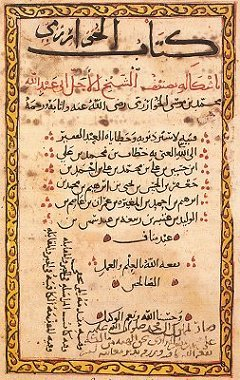
\includegraphics[width = 0.25 \textwidth]{media/buchAlChwarizmi.jpg}
\end{center}


\section{Mengen Terme und Gleichungen}
\subsection{Mengen}
\textbf{Einführungsfrage}: Welche Arten von Zahlen kennen Sie?

Bei gewissen Fragestellungen ist oft klar, dass man sich nur für eine bestimmte Art von Zahlen interessiert. Wenn man beispielsweise nach einer Streckenlänge fragt, kommen nur positive Zahlen infrage. Bei den Schulnoten hingegen kommen nur die Zahlen \(1, 1.5, 2, 2.5, \ldots\) bis \(6\) infrage. Für diese Fälle wurde der Begriff der Menge eingeführt.

\begin{definition}
    {Zahlenmenge}{}
    Eine Zahlenmenge \(M\) ist eine Zusammenfassung von bestimmten Zahlen.

    Gehört eine Zahl \(x\) zur Zahlenmenge \(M\), so sagt man, \(x\) ist \textbf{ein Element} der Menge \(M\) und schreibt dafür
    \[
        x \in M.
    \]
    Gehört eine Zahl \(x\) nicht zu einer Menge \(M\), so schreibt man
    \[
        x \notin M.
    \]

    Wenn eine Menge keine Elemente beinhaltet, spricht man von der leeren Menge
    \[
        \emptyset \qquad \text{oder} \qquad \{\}.
    \]

\end{definition}

Am einfachsten ist es wohl, wenn man sich eine Zahlenmenge als einen Sack vorstellt, der gewisse Zahlen enthält. Die leere Menge ist dann gewissermassen ein leerer Sack.

Wenn eine Menge nur wenige Zahlen enthält, kann sie durch \textit{Aufzählen} ihrer Elemente angegeben werden. Dafür schreibt man die Liste der Elemente in geschweiften Klammern. Die Menge der Schulnoten wäre dann
\[
    \{1, 1.5, 2, 2.5, \ldots, 6\}.
\]

Für Mengen mit vielen oder gar unendlich vielen Elementen ist die aufzählende Schreibweise ungünstig. Solche Mengen werden in der sogenannten \textit{beschreibenden Form} angegeben. Die Menge der Schulnoten wäre dann
\[
    \{x \mid 1 \leq x \leq 6,\; x \text{ ist ein Vielfaches von } 0.5\}.
\]

Der senkrechte Strich ist dabei eine Abkürzung für \enquote{mit der Eigenschaft, dass}.
\subsubsection{Wichtige Zahlenmengen}
Die natürlichen Zahlen sind jene Zahlen, die man beim Zählen verwendet:
\begin{definition}{Natürliche Zahlen}{natuerlichezahlen}
    Die Menge \(\mathbb{N}\) der natürlichen Zahlen ist die Menge
    \[ \N = \{1, 2, 3, 4, 5, \ldots\} \]
\end{definition}
Die Gemeinschaft der Mathematiker ist sich uneins, ob die Zahl \(0\) auch zu den natürlichen Zahlen gehören soll oder nicht. Bei uns wird sie standardmässig nicht dazugehören. Falls wir die Null benötigen, können wir die Zahlenmenge \(\mathbb{N}_0 = \{0, 1, 2, 3, 4, 5, \ldots\}\) betrachten.

\begin{definition}{Die ganzen Zahlen}{}
    Die Menge \(\mathbb{Z}\) der ganzen Zahlen ist definiert durch
    \[
        \mathbb{Z} = \{\ldots, -3, -2, -1, 0, 1, 2, 3, \ldots\}.
    \]

    Oder in beschreibender Form
    \[
        \mathbb{Z} = \{x \mid x \in \mathbb{N}_0 \text{ oder } -x \in \mathbb{N}\}.
    \]

    (Die beschreibende Form liest man so: \textit{\(\mathbb{Z}\) ist die Menge aller \(x\) mit der Eigenschaft, dass \(x\) in der Menge \(\mathbb{N}_0\) oder \(-x\) in der Menge \(\mathbb{N}\) liegt}.)
\end{definition}

\begin{definition}
    {Die rationale Zahlen}{}
    Das Resultat einer Division von zwei ganzen Zahlen nennt man einen (gewöhnlichen) Bruch.

    Die Menge \(\mathbb{Q}\) der rationalen Zahlen ist die Menge aller Brüche.
    \[
        \mathbb{Q}
        =
        \left\{
        \frac{a}{b}
        \;\middle|\;
        a \in \mathbb{Z}
        \text{ und }
        b \neq 0 \in \mathbb{Z}
        \right\}
    \]
\end{definition}

\textbf{Die reellen Zahlen \(\R\) }

Wenn Sie nun der Meinung sind, dass es jenseits der Brüche keine weiteren Zahlen gibt, sind Sie in bester Gesellschaft: Pythagoras (um 510 v.\,Chr. gestorben) war überzeugt, dass es gar keine anderen Zahlen als Brüche geben kann.

Als einer der Ersten hat wohl Hippasos von Metapont (ca.\ 500 v.\,Chr.) entdeckt, dass es Zahlen gibt, die sich nicht als Bruch schreiben lassen. Solche Zahlen nennt man auch \textit{irrational}. Zusammen mit den rationalen Zahlen bilden sie die Menge der reellen Zahlen:
\begin{definition}
    {Die reellen Zahlen \(\R\)}{}
    Die Menge \(\mathbb{R}\) der reellen Zahlen besteht aus allen rationalen und irrationalen Zahlen.
\end{definition}
Vielleicht haben Sie gemerkt, dass wir gar nicht genau festgelegt haben, was denn irrationale Zahlen sind. Eine genaue Definition der reellen Zahlen ist aber gar nicht so einfach. Siehe vielleicht später im Schwerpunktfach AM\dots

Wenn nichts anderes erwähnt wird, werden wir in der Mittelschule immer mit reellen Zahlen arbeiten. Diese können auf der sogenannten Zahlengerade angesiedelt werden: Jeder Zahl entspricht ein Punkt auf der Zahlengerade und umgekehrt.

\begin{center}
    \begin{tikzpicture}
        \draw[->] (-5,0) -- (6.7,0);
        \foreach \x in {-4,-3,...,6} {
                \draw (\x,0.08) -- (\x,-0.08) node[below] {\(\x\)};
            }
    \end{tikzpicture}
\end{center}

Weitere Zahlenmengen:
\[
    \mathbb{R}^{+}
    =
    \{x \in \mathbb{R} \mid x > 0\}
    \qquad
    \text{\enquote{positive reelle Zahlen}}
\]

\[
    \mathbb{R}^{-}_{0}
    =
    \{x \in \mathbb{R} \mid x \leq 0\}
    \qquad
    \text{\enquote{negative reelle Zahlen und Null}}
\]

analog \(\mathbb{Z}^{-}\), \(\mathbb{Q}^{+}_{0}\), usw.



\textbf{\textit{Rational oder irrational?}}

Woran erkennt man eigentlich, ob eine Zahl rational ist (also in \(\mathbb{Q}\) liegt)? Das ist ganz einfach! Die Dezimaldarstellung von Brüchen ist entweder endlich oder periodisch.

\begin{itemize}
    \item \(2.423\) ist eine rationale Zahl, weil die Dezimaldarstellung endlich ist
          \[
              \left(2.423 = \frac{2423}{1000}\right).
          \]

    \item \(2.753753753753753\ldots = 2.\overline{753}\) ist eine rationale Zahl, weil die Dezimaldarstellung periodisch ist
          \[
              \left(2.\overline{753} = \frac{2751}{999}\right).
          \]
          (Wie findet man wohl den dazugehörigen Bruch?)

    \item \(1.234567891011121314\ldots\) ist eine irrationale Zahl, weil sie weder endlich noch periodisch ist.
\end{itemize}

Der letzte Punkt tönt einfacher als er ist: Schliesslich kennt man bei einer Zahl wie \(\sqrt{2}\) nicht alle unendlich vielen Ziffern nach dem Dezimalpunkt. Bloss weil sich in den ersten paar Milliarden kein sich wiederholendes Muster zeigt, heisst das noch lange nicht, dass in der darauffolgenden Unendlichkeit kein solches auftreten wird.

Mehr zu diesem Thema werden wir im letzten Teilkapitel besprechen \dots

\clearpage

\begin{ueb}
    {Übungen zu den wichtigen Zahlenmengen}{zahlenmengen}

    \begin{enumerate}
        \item Kreuzen Sie an, in welchen der angegebenen Zahlenmengen die Zahlen enthalten sind. Tipp: Wir werden später sehen, dass \(\sqrt{5}\) eine irrationale Zahl ist.

              \[
                  \begin{array}{c|c|c|c|c|c|c|c|c|c|c}
                                   & \dfrac{2}{5}   & 7               & -1.5      & -\dfrac{8}{4} & \sqrt{5} & \sqrt{16}
                                   & 1.4 \cdot 10^3 & 2.04 \cdot 10^2 & \sqrt{-5} & -\sqrt{5}                                       \\ \hline
                      \mathbb{N}   &                &                 &           &               &          &           &  &  &  & \\ \hline
                      \mathbb{Z}   &                &                 &           &               &          &           &  &  &  & \\ \hline
                      \mathbb{Q}   &                &                 &           &               &          &           &  &  &  & \\ \hline
                      \mathbb{Q}^- &                &                 &           &               &          &           &  &  &  & \\ \hline
                      \mathbb{R}   &                &                 &           &               &          &           &  &  &  &
                  \end{array}
              \]

        \item
              Beantworten Sie die Frage oder beurteilen Sie, ob die Aussage wahr oder falsch ist.

              \begin{enumerate}
                  \item Sind die negativen gewöhnlichen Brüche in \(\mathbb{Q}\) enthalten?
                  \item Jede natürliche Zahl liegt auch in \(\mathbb{Z}\).
                  \item Eine natürliche Zahl gehört nicht zu \(\mathbb{Q}\), weil sie ja schon in \(\mathbb{N}\) ist.
                        %   \item Liegen alle Dezimalbrüche in \(\mathbb{Q}\)?  % nicht eindeutig. Sind nur endliche Dezimalbrüche gemeint?
                  \item Gehört jede Zahl in \(\mathbb{Q}\) auch zu \(\mathbb{R}\)?
              \end{enumerate}
        \item Beschreiben Sie in Worten, um welche Zahlen es sich handelt.

              \begin{enumerate}
                  \item \(\mathbb{Z}\) ohne \(\mathbb{N}\)
                  \item \(\mathbb{Z}\) ohne \(\{-1,-2,-3,\ldots\}\)
                  \item \(\mathbb{Q}^{+}\) ohne \(\{-1,-2,-3,\ldots\}\)
              \end{enumerate}
        \item Die folgenden Mengen sind in beschreibender Form angegeben. Geben Sie die Menge in aufzählender Form an.

              Zum Beispiel
              \[
                  \{n \in \mathbb{N} \mid 2n < 10\} = \{1,2,3,4\}.
              \]

              \begin{enumerate}
                  \item \(A = \{n \in \mathbb{N} \mid n \text{ ist ein Teiler von } 36\}\)
                  \item \(B = \{n \in \mathbb{N} \mid n < 10 \text{ und } n = 2k \text{ für eine Zahl } k \in \mathbb{N}\}\)
                  \item \(C = \{n \in \mathbb{N} \mid n^2 \leq 100\}\)
                  \item \(D = \{x \in \mathbb{Z} \mid -3 \leq x - 5 \leq 3\}\)
              \end{enumerate}

        \item Die folgenden Mengen sind in aufzählender Form angegeben. Geben Sie die Menge in beschreibender Form an.

              \begin{enumerate}
                  \item \(A = \{1,8,27,64,125\}\)
                  \item \(B = \{3,4,5,6,7,8,9,10\}\)
                  \item \(C = \{1,3,5,7,9,11\}\)
                  \item \(D = \{1,2,3,4,6,12\}\)
              \end{enumerate}
        \item Challenge:
              \begin{enumerate}
                  \item Erklären Sie, wie man den Bruch für die Zahl \(x = 2.\overline{753}\) findet. Tipp: Betrachten Sie die Zahl \(1000\cdot x\) und die Zahl \(x\) und berechnen Sie damit die Zahl \(999\cdot x\).
                  \item Finden Sie einen Bruch für die Zahl \(x = 1.234\overline{34}\).
              \end{enumerate}
    \end{enumerate}


\end{ueb}



\clearpage
\emph{Lösungen:}

\begin{enumerate}
    \item
          \[
              \begin{array}{c|c|c|c|c|c|c|c|c|c|c}
                               & \dfrac{2}{5}   & 7               & -1.5      & -\dfrac{8}{4} & \sqrt{5} & \sqrt{16}
                               & 1.4 \cdot 10^3 & 2.04 \cdot 10^2 & \sqrt{-5} & -\sqrt{5}                            \\ \hline
                  \mathbb{N}   &                & \times          &           &               &          & \times
                               & \times         & \times          &           &                                      \\ \hline
                  \mathbb{Z}   &                & \times          &           & \times        &          & \times
                               & \times         & \times          &           &                                      \\ \hline
                  \mathbb{Q}   & \times         & \times          & \times    & \times        &          & \times
                               & \times         & \times          &           &                                      \\ \hline
                  \mathbb{Q}^- &                &                 & \times    & \times        &          &
                               &                &                 &           &                                      \\ \hline
                  \mathbb{R}   & \times         & \times          & \times    & \times        & \times   & \times
                               & \times         & \times          &           & \times
              \end{array}
          \]

    \item
          \begin{enumerate}
              \item Ja.
              \item Wahr.
              \item Falsch.
                    %   \item Wahr. % Falls endliche Dezimalbrüche gemeint sind.
              \item Ja.
          \end{enumerate}

    \item
          \begin{enumerate}
              \item Die ganzen Zahlen kleiner oder gleich \(0\).
              \item Die nichtnegativen ganzen Zahlen, also \(\mathbb{N}_0\).
              \item Die positiven rationalen Zahlen, also \(\mathbb{Q}^+\).
          \end{enumerate}

    \item
          \begin{enumerate}
              \item \(A = \{1,2,3,4,6,9,12,18,36\}\)
              \item \(B = \{2,4,6,8\}\)
              \item \(C = \{1,2,3,4,5,6,7,8,9,10\}\)
              \item \(D = \{2,3,4,5,6,7,8\}\)
          \end{enumerate}

    \item
          \begin{enumerate}
              \item \(A = \{n^3 \mid n \in \mathbb{N},\ n \leq 5\}\)
              \item \(B = \{n \in \mathbb{N} \mid 3 \leq n \leq 10\}\)
              \item \(C = \{n \in \mathbb{N} \mid n < 12 \text{ und } n \text{ ungerade}\}\)
              \item \(D = \{n \in \mathbb{N} \mid n \text{ ist ein Teiler von } 12\}\)
          \end{enumerate}

    \item \begin{enumerate}
              \item \(\frac{917}{333}\)
              \item \(\frac{611}{495}\)
          \end{enumerate}
          %       \begin{enumerate}
          %           \item
          %                 \[
          %                     1000x = 2753.\overline{753},
          %                     \qquad
          %                     x = 2.\overline{753}
          %                 \]
          %                 \[
          %                     999x = 2751
          %                     \qquad\Longrightarrow\qquad
          %                     x = \frac{2751}{999}
          %                     = \frac{917}{333}.
          %                 \]

          %           \item
          %                 \[
          %                     100000x - 1000x = 122200
          %                 \]
          %                 \[
          %                     99000x = 122200
          %                     \qquad\Longrightarrow\qquad
          %                     x = \frac{122200}{99000}
          %                     = \frac{611}{495}.
          %                 \]
          % \end{enumerate}
\end{enumerate}



\clearpage

\subsubsection{Mengenoperationen und Teilmengen}
Vergleicht man die Elemente der Mengen \(\mathbb{Z}\) und \(\mathbb{N}\), so stellt man fest, dass alle Elemente von \(\mathbb{N}\) auch in \(\mathbb{Z}\) enthalten sind. Man sagt dann, dass \(\mathbb{N}\) eine Teilmenge von \(\mathbb{Z}\) ist:

\begin{definition}{Teilmenge}{teilmenge}
    Eine Menge \(A\) heisst \textit{Teilmenge} einer Menge \(B\), wenn alle Elemente von \(A\) auch in der Menge \(B\) liegen.

    Schreibweise:
    \[
        A \subset B
    \]

    \begin{center}
        \begin{tikzpicture}[scale=0.8]
            \draw (0,0) circle (1.8);
            \draw (-0.25,-0.25) circle (1.0);
            \node at (0,0) {\(A\)};
            \node at (0.9,1.1) {\(B\)};
        \end{tikzpicture}
    \end{center}
\end{definition}

Bemerkung: Ist \(A\) keine Teilmenge von \(B\), schreibt man
\[
    A \not\subset B.
\]

\textbf{Beispiel:}
\[
    \mathbb{Z} \subset \mathbb{R}.
\]

\begin{definition}{Schnittmenge}{schnittmenge}
    Die \textit{Schnittmenge} der Mengen \(A\) und \(B\) ist diejenige Menge, die alle Elemente enthält, welche in \(A\) und in \(B\) enthalten sind.

    Schreibweise für Schnittmengen:
    \[
        A \cap B
    \]

    Es gilt:
    \[
        A \cap B = \{x \mid x \in A \text{ und } x \in B\}.
    \]

    \begin{center}
        \begin{tikzpicture}
            \begin{scope}
                \clip (-1,0) circle (1.2);
                \fill[gray!40] (1,0) circle (1.2);
            \end{scope}
            \draw (-1,0) circle (1.2);
            \draw (1,0) circle (1.2);
            \node at (-1.4,0) {\(A\)};
            \node at (1.4,0) {\(B\)};
        \end{tikzpicture}
    \end{center}
\end{definition}

\textbf{Beispiel einer Schnittmenge:}
\[
    \{\text{Primzahlen}\}
    \cap
    \{\text{natürliche Zahlen kleiner als } 10\}
    =
    \{2,3,5,7\}.
\]

\begin{definition}{Vereinigungsmenge}{vereinigungsmenge}
    Die \textit{Vereinigungsmenge} der Mengen \(A\) und \(B\) ist diejenige Menge, die alle Elemente enthält, die in der Menge \(A\) oder \(B\) enthalten sind.

    Schreibweise für Vereinigungsmengen:
    \[
        A \cup B
    \]

    Es gilt:
    \[
        A \cup B = \{x \mid x \in A \text{ oder } x \in B\}.
    \]

    \begin{center}
        \begin{tikzpicture}
            \fill[gray!40] (-1,0) circle (1.2);
            \fill[gray!40] (1,0) circle (1.2);
            \draw (-1,0) circle (1.2);
            \draw (1,0) circle (1.2);
            \node at (-1.4,0) {\(A\)};
            \node at (1.4,0) {\(B\)};
        \end{tikzpicture}
    \end{center}
\end{definition}

\textbf{Beispiel einer Vereinigungsmenge:}
\[
    \{\text{Teiler von } 6\}
    \cup
    \{x \mid x \in \mathbb{N} \text{ und } 4 < x < 8\}
    =
    \{1,2,3,5,6,7\}.
\]

\begin{definition}{Differenzmenge}{differenzmenge}
    Die \textit{Differenzmenge} der Mengen \(A\) und \(B\) ist diejenige Menge, die alle Elemente enthält, die in der Menge \(A\), aber nicht in der Menge \(B\) enthalten sind.

    Schreibweise für Differenzmengen:
    \[
        A \setminus B
    \]

    Es gilt:
    \[
        A \setminus B
        =
        \{x \mid x \in A \text{ und } x \notin B\}.
    \]

    \begin{center}
        \begin{tikzpicture}
            \begin{scope}
                \clip (-1,0) circle (1.2);
                \fill[gray!40] (-1,0) circle (1.2);
                \fill[gray!10] (1,0) circle (1.2);
            \end{scope}
            \draw (-1,0) circle (1.2);
            \draw (1,0) circle (1.2);
            \node at (-1.4,0) {\(A\)};
            \node at (1.4,0) {\(B\)};
        \end{tikzpicture}
    \end{center}
\end{definition}

\textbf{Beispiel einer Differenzmenge:}
\[
    \{\text{Teiler von } 6\}
    \setminus
    \{\text{Primzahlen}\}
    =
    \{1,6\}.
\]

In Anwendungssituationen wird häufig nur ein beschränkter Bereich der reellen Zahlen betrachtet. Wenn die Variable \(v\) die Schnelligkeit eines Teilchens in \(\mathrm{m/s}\) beschreibt, so ist \(v\) eine reelle Zahl zwischen Null und der Lichtgeschwindigkeit \(c \cong 299'792'458\).

In der Sprache der Mathematik würde man sagen: \(v\) liegt im \textbf{Intervall} \([0,c]\).

\begin{definition}{Intervalle}{intervalle}
    \textbf{Intervalle} sind Mengen von reellen Zahlen zwischen zwei Grenzen. Je nachdem, ob die eckigen Klammern nach innen oder aussen zeigen, gehören die Grenzen zur Menge oder nicht. Für \(a<b\) gilt:
    \[
        \begin{aligned}
            [a,b]                                                & = \{x \in \mathbb{R} \mid a \leq x \leq b\}, \\
            ]a,b[                                                & = \{x \in \mathbb{R} \mid a < x < b\},       \\
            [a,b[   &= \{x \in \mathbb{R} \mid a \leq x < b\},\\
                    ]a,b] & = \{x \in \mathbb{R} \mid a < x \leq b\}.
        \end{aligned}
    \]
\end{definition}

\textbf{Speziell:} Man kann mit der Intervallschreibweise auch unbeschränkte Mengen angeben. Die Menge aller reellen Zahlen, die grösser oder gleich \(5\) sind, wäre zum Beispiel
\[
    M = [5,\infty[.
\]

Analog ist
\[
    ]-\infty,10[
\]
die Menge aller reellen Zahlen, die kleiner als \(10\) sind.

Oder im Extremfall:
\[
    \mathbb{R} = ]-\infty,\infty[.
\]

Merke: Bei \(\infty\) zeigt die Klammer immer gegen aussen.

\begin{bsp}
    {}{}
    \[ [-2, 2 [ \, \cap \, ]0, 3] = ? \]
    \vspace*{5 cm}
\end{bsp}







\clearpage

\begin{ueb}
    {Zu Mengenoperationen und Intervalle}{}
    \begin{enumerate}
        \item Setzen Sie für \(\diamond\) das richtige Zeichen
              \(\left(\in,\notin,\subset,\not\subset\right)\) ein.

              \begin{enumerate}
                  \item \(\mathbb{Z} \diamond \mathbb{Q}\)
                  \item \(\mathbb{Z} \diamond \mathbb{N}\)
                  \item \(-5 \diamond \mathbb{N}\)
                  \item \(-5 \diamond \mathbb{Q}\)
                  \item \(\{2,7\} \diamond \mathbb{N}\)
                  \item \(\{0,\pm1,\pm2,\pm3,\ldots\} \diamond \mathbb{Z}\)
              \end{enumerate}

        \item Gegeben sind die Mengen
              \[
                  A=\{11,13,15,17,18\}
                  \qquad\text{und}\qquad
                  B=\{10,12,13,14,16\}.
              \]
              Bestimmen Sie:

              \begin{enumerate}
                  \item \(A \cup B\)
                  \item \(A \cap B\)
                  \item \(A \setminus B\)
                  \item \(B \setminus A\)
                  \item \((A \setminus B)\cup(B \setminus A)\)
                  \item \((A \cup B)\setminus(A \cap B)\)
              \end{enumerate}

        \item Setzen Sie für \(\diamond\) das richtige Zeichen
              \(\left(\in,\notin,\subset,\not\subset\right)\) ein.

              \begin{enumerate}
                  \item \(b \diamond \{a,b,c,d,e,f\}\)
                  \item \(\{b\} \diamond \{a,b,c,d,e,f\}\)
                  \item \(\{b,d,g\} \diamond \{a,b,c,d,e,f\}\)
                  \item \(g \diamond \{a,b,c,d,e,f\}\)
                  \item \(\{a,b,c,d,e\} \diamond \{a,b,c\}\)
                  \item \(\{b,c,d,e\} \diamond \{b,c,d,e\}\)
              \end{enumerate}

        \item Beurteilen Sie, ob die Aussage wahr oder falsch ist.

              \begin{enumerate}
                  \item \((A \cup B) \subset B\)
                  \item \((A \cap B) \subset B\)
                  \item \(A \subset (A \cup B)\)
                  \item \(A \subset (A \cap B)\)
              \end{enumerate}
        \item Geben Sie die folgenden Mengen als ein Intervall an:

              \begin{enumerate}
                  \item \(A = \{x \in \mathbb{R} \mid -5 < x \leq 3\}\)
                  \item \(B = \{x \in \mathbb{R} \mid 1 < x < 2.5\}\)
                  \item \(C = \{x \in \mathbb{R} \mid x < 1\}\)
                  \item \(D = [-1,5] \cup [4,6[\)
                  \item \(E = [-1,5] \cap [4,6[\)
                  \item \(F = [-2,8] \setminus [5,9]\)
              \end{enumerate}
    \end{enumerate}
\end{ueb}


\emph{Lösungen:}
\begin{enumerate}
    \item
          \begin{enumerate}
              \item \(\mathbb{Z} \subset \mathbb{Q}\)
              \item \(\mathbb{Z} \not\subset \mathbb{N}\)
              \item \(-5 \notin \mathbb{N}\)
              \item \(-5 \in \mathbb{Q}\)
              \item \(\{2,7\} \subset \mathbb{N}\)
              \item \(\{0,\pm1,\pm2,\pm3,\ldots\} \subset \mathbb{Z}\)
          \end{enumerate}

    \item
          \begin{enumerate}
              \item \(A \cup B = \{10,11,12,13,14,15,16,17,18\}\)
              \item \(A \cap B = \{13\}\)
              \item \(A \setminus B = \{11,15,17,18\}\)
              \item \(B \setminus A = \{10,12,14,16\}\)
              \item \((A \setminus B)\cup(B \setminus A) = \{10,11,12,14,15,16,17,18\}\)
              \item \((A \cup B)\setminus(A \cap B) = \{10,11,12,14,15,16,17,18\}\)
          \end{enumerate}

    \item
          \begin{enumerate}
              \item \(b \in \{a,b,c,d,e,f\}\)
              \item \(\{b\} \subset \{a,b,c,d,e,f\}\)
              \item \(\{b,d,g\} \not\subset \{a,b,c,d,e,f\}\)
              \item \(g \notin \{a,b,c,d,e,f\}\)
              \item \(\{a,b,c,d,e\} \not\subset \{a,b,c\}\)
              \item \(\{b,c,d,e\} \subset \{b,c,d,e\}\)
          \end{enumerate}

    \item
          \begin{enumerate}
              \item Falsch.
              \item Wahr.
              \item Wahr.
              \item Falsch.
          \end{enumerate}

    \item
          \begin{enumerate}
              \item \(A = ]-5,3]\)
              \item \(B = ]1,2.5[\)
              \item \(C = ]-\infty,1[\)
              \item \(D = [-1,6[\)
              \item \(E = [4,5]\)
              \item \(F = [-2,5[\)
          \end{enumerate}
\end{enumerate}




\clearpage


\subsubsection{Rationale und irrationale Zahlen}

In diesem Abschnitt werden wir den Unterschied zwischen rationalen und irrationalen Zahlen genauer untersuchen. Dabei werden wir die folgenden drei Fragen diskutieren:
\begin{itemize}
    \item Wieso kann man jede periodische Dezimalzahl als Bruch schreiben?
    \item Wieso ist die Dezimaldarstellung einer rationalen Zahl entweder endlich oder periodisch?
    \item Wie kann man zeigen, dass eine Zahl wie \(\sqrt{2}\) irrational ist?
\end{itemize}

Die erste Frage haben Sie vielleicht bereits in der Übung \Cref{uebng:zahlenmengen} beantwortet: Durch geschicktes Rechnen kann man bei einer solchen Zahl zum Beispiel \( x = 2.\overline{753}\) die Nachkommastellen eliminieren. In diesem Fall rechnet man:
\[
    1000x = 2753.\overline{753},
    \qquad
    x = 2.\overline{753}
\]
Damit erhält man:
\[
    999x = 2751
    \qquad\Longrightarrow\qquad
    x = \frac{2751}{999}
    = \frac{917}{333}.
\]

Man kann sich leicht überlegen, dass man auf diese Weise jede periodische Zahl als Bruch darstellen kann.

Zur zweiten Frage:

\begin{LA}
    {Brüche haben eine periodische Dezimaldarstellung}{}
    Die folgenden Aufgaben sollen Ihnen helfen zu verstehen, wieso jeder Bruch eine periodische (oder endliche) Dezimaldarstelung hat.
    \begin{enumerate}
        \item Finden Sie die Dezimaldarstellung von \(\frac{1}{7}\), indem Sie schriftlich dividieren:
              \begin{align*}
                   & 1.00000 : 7 = 0.1\ldots \\
                   & 10                      \\
                   & \phantom{1}30
              \end{align*}
              \vspace*{2 cm}
        \item 	Wann beginnt sich die Dezimaldarstellung zu wiederholen? Wie viele verschiedene Reste kann es bei einer Division durch eine ganze Zahl \(n\) geben?
        \item 	Wieso ist die Dezimaldarstellung von \(\frac{1}{n}\) endlich oder periodisch? Wie lang kann die Periode sein?
    \end{enumerate}
\end{LA}












\clearpage

Nachdem wir die ersten beiden Fragen beantwortet haben, ist klar, dass die rationalen Zahlen genau die Zahlen sind, deren Dezimaldarstellung endlich oder periodisch ist. So kann man sich leicht eine irrationale Zahl denken. Zum Beispiel ist die Zahl \(1.234567891011121314\ldots\) irrational, weil sie weder endlich noch periodisch ist.

Für die Mathematiker der Antike ist das kein gültiges Argument für die Existenz von irrationalen Zahlen. Zum Einen weil sie nicht ein Stellenwertsystem zur Darstellung der Zahlen verwendet haben, sondern ein System, das ähnlich wie die römischen Zahlen funktioniert hat. Zum Anderen weil Zahlen im antiken Griechenland als Längen von Strecken gedacht wurden. Umso mehr erstaunte es die damaligen Mathematiker als Strecken entdeckt wurden, deren Längen nicht als Bruch dargestellt werden können.

Im Folgenden werden wir den Beweis von Euklid nachvollziehen, dass die Zahl \(\sqrt{2}\) irrational ist. Diese Zahl entspricht der Länge der Diagonale eines Quadrats mit Seitenlänge 1. Wir werden dazu einige Vorbereitungsaufgaben lösen.


\begin{LA}
    {Vorbereitung auf den Beweis von Euklid}{}
    \begin{enumerate}
        \item Zerlegen Sie folgende Zahlen in Primfaktoren:

              Beispiel: \(48 = 2^4 \cdot 3\)

              \begin{enumerate}
                  \item \(6\)
                  \item \(15\)
                  \item \(20\)
                  \item \(36\)
                  \item  \(225\)
                  \item \(400\)
              \end{enumerate}

              Wie hängen die ersten drei Zahlen mit den letzten drei zusammen? Wie hängen deren Primfaktorzerlegungen zusammen?

        \item Betrachten Sie die Aussage:

              \textit{In der Primfaktorzerlegung einer Quadratzahl kommt der Primfaktor \(2\) entweder gar nicht oder in gerader Anzahl vor.}

              Erklären Sie in eigenen Worten, wieso die Aussage stimmt.
    \end{enumerate}
\end{LA}

\clearpage
Der Beweis von Euklid ist ein sogenannter \textit{Widerspruchsbeweis}. Bei dieser Beweismethode geht man wie folgt vor:

\begin{enumerate}
    \item Man nimmt an, dass die Behauptung falsch ist. (\textit{Widerspruchsannahme})
    \item Man zeigt, dass die Annahme, die Behauptung sei falsch, zu einem Widerspruch führt.
    \item Man folgert aus 2., dass die Behauptung stimmen muss.
\end{enumerate}

\begin{satz}{Irrationalität von \(\sqrt{2}\)}{}
    Die Zahl \(\sqrt{2}\) ist irrational (also kein Bruch).
\end{satz}








\clearpage

\begin{ueb}
    {Zur rationale und irrationale Zahlen}{Q vs R}
    \begin{enumerate}
        \item
              Verwandeln Sie den periodischen Dezimalbruch in einen gewöhnlichen Bruch.
              \begin{enumerate}
                  \item \(0.\overline{543}\)
                  \item \(0.25\overline{7}\)
                  \item \(0.4\overline{81}\)
              \end{enumerate}


        \item
              \begin{enumerate}
                  \item Beweisen Sie wie im Theoriebeispiel, dass \(\sqrt{3}\) irrational ist.
                  \item Weisen Sie nach, dass \(\sqrt{20}\) irrational ist.
                  \item \(\sqrt{25}=5\) ist eine aufgehende Quadratwurzel und somit rational.
                        Erklären Sie, warum das bei \(\sqrt{2}\) verwendete Widerspruchsargument
                        bei \(\sqrt{25}\) nicht zu einem Widerspruch führt.
              \end{enumerate}

        \item Wie können Sie anhand der Primfaktorzerlegung der natürlichen Zahl \(n\) erkennen, ob auch \(\sqrt{n}\) eine natürliche Zahl ist?


        \item Ist die Aussage wahr oder falsch? Begründen Sie.

              \begin{enumerate}
                  \item \(4+\sqrt{7}\) ist rational.
                  \item Die Summe zweier irrationaler Zahlen kann rational sein.
                  \item Summe, Differenz, Produkt sowie Quotient zweier rationaler Zahlen sind rational.
                  \item Das Produkt und der Quotient zweier irrationaler Zahlen sind auch irrational.
              \end{enumerate}

    \end{enumerate}
\end{ueb}

\clearpage
\emph{Lösungen:}

\begin{enumerate}
    \item
          \begin{enumerate}
              \item \(\frac{181}{333}\)
              \item \(\frac{58}{225}\)
              \item \(\frac{53}{110}\)
          \end{enumerate}

    \item \dots
          %   \begin{enumerate}
          %       \item Angenommen, \(\sqrt{3}=\frac{a}{b}\). Dann
          %             \[
          %                 3b^2=a^2.
          %             \]
          %             Links kommt der Primfaktor \(3\) in ungerader, rechts in gerader Anzahl vor. Widerspruch. Also ist \(\sqrt{3}\) irrational.

          %       \item
          %             \[
          %                 20=2^2\cdot5.
          %             \]
          %             In der Primfaktorzerlegung von \(20\) kommt der Primfaktor \(5\) in ungerader Anzahl vor. Daher kann \(20\) keine Quadratzahl sein und \(\sqrt{20}\) ist irrational.

          %       \item Es entsteht kein Widerspruch, denn
          %             \[
          %                 25=5^2
          %             \]
          %             enthält jeden Primfaktor in gerader Anzahl. Tatsächlich gilt beispielsweise
          %             \[
          %                 \sqrt{25}=\frac{5}{1}.
          %             \]
          %   \end{enumerate}

    \item \dots %\(\sqrt{n}\) ist genau dann eine natürliche Zahl, wenn in der Primfaktorzerlegung von \(n\) jeder Primfaktor in gerader Anzahl vorkommt.

    \item \dots
          %   \begin{enumerate}
          %       \item Falsch, da \(\sqrt{7}\) irrational ist und somit auch \(4+\sqrt{7}\) irrational ist.

          %       \item Wahr, zum Beispiel
          %             \[
          %                 \sqrt{2}+(-\sqrt{2})=0.
          %             \]

          %       \item Wahr, wobei beim Quotienten der Divisor ungleich \(0\) sein muss.

          %       \item Falsch, zum Beispiel
          %             \[
          %                 \sqrt{2}\cdot\sqrt{2}=2
          %                 \qquad\text{und}\qquad
          %                 \frac{\sqrt{2}}{\sqrt{2}}=1.
          %             \]
          %   \end{enumerate}
\end{enumerate}
































\clearpage
\subsection{Terme}
\begin{LA}
    {Einführungsfrage}{}

    Denken Sie sich heimlich eine beliebige Zahl und verraten Sie diese niemandem.

    \begin{enumerate}
        \item Addieren Sie \(4\).
        \item Multiplizieren Sie das Ergebnis mit \(5\).
        \item Subtrahieren Sie das Dreifache Ihrer ursprünglich gedachten Zahl.
        \item Subtrahieren Sie \(6\).
        \item Teilen Sie das Ergebnis durch \(2\).
        \item Subtrahieren Sie Ihre ursprünglich gedachte Zahl.
    \end{enumerate}

    \textbf{Notieren Sie nur Ihr Endresultat.}

    Vergleichen Sie das Resultat mit der*m Nachbar*in.

    Was fällt Ihnen auf? Finden Sie eine Erklärung.
\end{LA}

\clearpage
\begin{LA}
    {Weitere Einführungsfragen}{}
    \begin{enumerate}
        \item
              \[
                  A = x^2 - xy + y^2,
                  \qquad
                  B = x^2 + y(y-x)
              \]

              \begin{enumerate}
                  \item Berechnen Sie den Wert von \(A\), wenn \(x=1\) und \(y=2\) ist.
                  \item Berechnen Sie den Wert von \(B\), wenn \(x=1\) und \(y=2\) ist.
                  \item Gibt es Zahlen \(x\) und \(y\), für welche \(A\) und \(B\) einen unterschiedlichen Wert liefern?
              \end{enumerate}

        \item
              \[
                  C = y(y+1)-x,
                  \qquad
                  D = 2xy+x
              \]

              \begin{enumerate}
                  \item Berechnen Sie den Wert von \(C\), wenn \(x=1\) und \(y=2\) ist.
                  \item Berechnen Sie den Wert von \(D\), wenn \(x=1\) und \(y=2\) ist.
                  \item Gibt es Zahlen \(x\) und \(y\), für welche \(C\) und \(D\) einen unterschiedlichen Wert liefern?
              \end{enumerate}

        \item (Diese Aufgabe kann für Schüler aus der zweiten Sek eventuell etwas schwierig sein.)

              Wird vom Produkt zweier Zahlen deren Summe subtrahiert und anschliessend \(1\) addiert, so ergibt sich das Produkt aus der um \(1\) verminderten ersten und der um \(1\) verminderten zweiten Zahl.

              Stimmt das?

        \item Challenge: Ein etwas anderer \enquote{Zaubertrick}. Finden Sie heraus, wie er funktioniert?

              Denken Sie sich eine Zahl. Addieren Sie dazu die Anzahl Ihrer Geschwister. Multiplizieren Sie die erhaltene Zahl mit neun. Wenn Sie gerne jassen, addieren Sie \(36\) zum Resultat. Bilden Sie die Quersumme der Quersumme der Quersumme der erhaltenen Zahl. Wenn das Zwischenresultat kleiner als fünf ist, addieren Sie drei, andernfalls subtrahieren Sie drei.

              Wieso erhält man mit dieser Rechnung immer sechs?
    \end{enumerate}
\end{LA}

\clearpage
Ein \textbf{Term} ist eine sinnvolle Zusammensetzung von Zahlen, Operationszeichen (\(+,-,\cdot,/\)), Klammern und Variablen. Letztere werden durch Buchstaben bezeichnet. Sie dienen als Stellvertreter für Zahlen.

Ein \textbf{Beispiel} für einen Term wäre
\[
    a^2+2ab^2+b^2.
\]
Für die Variablen \(a\) und \(b\) können Zahlen eingesetzt werden. Setzt man beispielsweise \(a=3\) und \(b=2\), so hat der Term den Wert \(37\). Für \(a=1\) und \(b=-1\) hat der Term den Wert \(4\).

Ein \textbf{anderes Beispiel} wäre der Term
\[
    a^2+b^2\cdot(1+2a).
\]
Wieder können wir den Variablen Zahlenwerte geben, zum Beispiel wieder \(a=3\) und \(b=2\). Der Term hat dann wiederum den Wert \(37\). Auch für den Fall, dass \(a=1\) und \(b=-1\) ist, liefert der zweite Term den gleichen Wert wie der erste (nämlich \(4\)).

Tatsächlich liefern die beiden Terme
\[
    a^2+2ab^2+b^2
    \qquad\text{und}\qquad
    a^2+b^2\cdot(1+2a)
\]
immer die gleichen Werte, unabhängig davon, welche Zahlen wir für \(a\) und \(b\) einsetzen.

\begin{definition}{Äquivalente Terme}{aequivalenteterme}
    Setzt man in zwei Terme jeweils die gleichen Zahlen für die Variablen ein und erhält man dabei für jede beliebige Einsetzung übereinstimmend das gleiche Ergebnis, heissen die zwei Terme \textbf{äquivalent}\footnote{Äquivalent heisst wörtlich \enquote{gleichwertig}: \enquote{äqui = gleich} und \enquote{valent = wertig}}.
\end{definition}

Im Beispiel der Terme \(a^2+2ab^2+b^2\) und \(a^2+b^2(1+2a)\) kann man leicht einsehen, dass sie äquivalent sind. Dazu genügt es, den zweiten Term auszumultiplizieren und neu zu ordnen:
\[
    a^2+b^2(1+2a)
    = a^2+b^2+b^2\cdot2a
    = a^2+2ab^2+b^2.
\]

Wichtig bei diesen Umformungsschritten ist, dass die Terme links und rechts des Gleichheitszeichens äquivalent sind.

\begin{definition}{Termumformungen}{termumformungen}
    Umformungen eines Terms in einen äquivalenten Term heissen \textbf{Termumformungen}.
\end{definition}

Beim Umformen von Termen werden die Grundgesetze der Arithmetik verwendet:

\[
    \begin{array}{l|c|c}
         & \text{Addition } +                 & \text{Multiplikation } \cdot \\ \hline
        \text{Kommutativgesetz K}
         & a+b=b+a
         & a\cdot b=b\cdot a                                                 \\ \hline
        \text{Assoziativgesetz A}
         & a+(b+c)=(a+b)+c
         & a\cdot(b\cdot c)=(a\cdot b)\cdot c                                \\ \hline
        \text{Neutrales Element N}
         & a+0=a
         & a\cdot1=a                                                         \\ \hline
        \text{Inverses Element I}
         & a+(-a)=(-a)+a=0
         & a\cdot\frac{1}{a}=1                                               \\ \hline
        \text{Distributivgesetz D}
         & \multicolumn{2}{c}{a(b+c)=ab+ac}
    \end{array}
\]

Das mag überraschen, weil in der Praxis viele andere Rechenregeln verwendet werden. \enquote{Minus mal Minus = Plus}, \enquote{steht ein Minus vor der Klammer, müssen alle Vorzeichen gewechselt werden}, \enquote{Null mal etwas = 0}, \enquote{Beim Multiplizieren von Brüchen rechnet man Zähler mal Zähler und Nenner mal Nenner} und viele mehr.

Tatsächlich sind alle diese Regeln direkte Folgerungen aus den Grundgesetzen der Arithmetik. Stellvertretend für alle anderen zeigen wir hier, wie man die Regel \enquote{Minus vor der Klammer} aus den Grundgesetzen herleiten kann:

\begin{satz}{Minus vor der Klammer}{minusvorderklammer}
    \[
        -(a+b)=-a-b
    \]
\end{satz}

\begin{proof}

    \[
        \begin{aligned}
            (a+b) + (-a - b) & \stackrel{A+}{=} a+b-a-b     \\
                             & \stackrel{K+}{=} a-a+b-b     \\
                             & \stackrel{A+}{=} (a-a)+(b-b) \\
                             & \stackrel{I+}{=} 0+0         \\
                             & \stackrel{N+}{=} 0.
        \end{aligned}
    \]
    Daraus folgt, dass \(-a-b\) das additive Inverse von \(a+b\) ist. Da das additive Inverse eindeutig ist, folgt daraus die Behauptung.
\end{proof}
%         -(a+(-b))
%          & \stackrel{N+}{=} -(a+(-b))+0                             \\
%          & \stackrel{I+}{=} -(a+(-b))+(a+(-a))                      \\
%          & \stackrel{N+}{=} \bigl(-(a+(-b))+(a+(-a))\bigr)+0        \\
%          & \stackrel{I+}{=} \bigl(-(a+(-b))+(a+(-a))\bigr)+(b+(-b)) \\
%          & \stackrel{A+}{=} -(a+(-b))+a+(-a)+b+(-b)                 \\
%          & \stackrel{K+}{=} -(a+(-b))+a+(-b)+(-a)+b                 \\
%          & \stackrel{A+}{=} \bigl(-(a+(-b))+(a+(-b))\bigr)+(-a)+b   \\
%          & \stackrel{I+}{=} 0+(-a)+b                                \\
%          & \stackrel{N+}{=} (-a)+b.
%     \end{aligned}
% \]

Aus theoretischer Sicht ist es eine interessante Erkenntnis, dass es zur Erklärung der Arithmetik eigentlich nur neun Regeln bedarf. Auch ist es einmal spannend zu sehen, wie man eine andere Rechenregel auf die Grundregeln zurückführt, aber: Beim Beweis merkt man, dass Termumformungen sehr umständlich werden, wenn man bloss auf die 9 Grundrechenregeln zurückgreift. Aus diesem Grund werden in der Praxis doch einige Regeln verwendet, mit denen man Rechenschritte überspringen kann -- eben wie jene, die wir gerade bewiesen haben. Damit kann man Terme schneller vereinfachen. Zum Beispiel
\[
    \begin{aligned}
        a(a+b)-(b^2-a^2)
         & = a^2+ab-b^2+a^2 \\
         & = 2a^2+ab-b^2.
    \end{aligned}
\]

Eine weitere nützliche Regel betrifft das Ausmultiplizieren von zwei Klammern:

\begin{satz}{Jede mit jeder}{jedemitjeder}
    \[
        (a+b)(c+d)=ac+ad+bc+bd
    \]
\end{satz}

\textbf{Beispiele:}

\begin{itemize}
    \item \((2x+1)(3x+2)=\)

    \item Auch mit negativen Vorzeichen:

          \(
          (3x-2)(3-4z)=
          \)

    \item Auch mit mehr als zwei Variablen:

          \(
          (a+b-c)(x+2y+2z)=
          \)
\end{itemize}


Speziell seien an dieser Stelle auch die Rechenregeln rund um Potenzen erwähnt. Zur Erinnerung:

\begin{definition}{Potenzen}{potenzen}
    Sei \(a \in \mathbb{R}\) und \(n \in \mathbb{N}\). Die Zahl \(a^n\) ist definiert als
    \[
        a^n
        =
        \underbrace{a \cdot a \cdot a \cdot \ldots \cdot a}_{n\text{ Faktoren}}.
    \]

    Speziell: \(a^1=a\)
\end{definition}

Damit ist zum Beispiel
\[
    a^3=a\cdot a\cdot a
    \qquad\text{und}\qquad
    a^4=a\cdot a\cdot a\cdot a
\]
und damit folgt:
\[
    a^3\cdot a^4=
\]

Oder ganz allgemein:
\[
    a^n\cdot a^m=
\]

Analog ist
\[
    \frac{a^5}{a^2}=
\]

Und
\[
    (a^2)^3=
\]

Und
\[
    (ab)^3=
\]

Allgemein gelten für Potenzen die folgenden Regeln:

\begin{satz}{Potenzgesetze}{potenzgesetze}
    Für \(a,b\in\mathbb{R}\) und \(n,m\in\mathbb{N}\) gilt:
    \begin{enumerate}
        \item
              \[
                  a^n\cdot a^m=a^{n+m}
                  \qquad\text{und}\qquad
                  \frac{a^n}{a^m}=a^{n-m}
              \]
              falls \(a\neq0\) und \(n>m\).

        \item
              \[
                  (a^n)^m=a^{n\cdot m}.
              \]

        \item
              \[
                  a^n\cdot b^n=(ab)^n
                  \qquad\text{und}\qquad
                  \frac{a^n}{b^n}
                  =
                  \left(\frac{a}{b}\right)^n
              \]
              falls \(b\neq0\).
    \end{enumerate}
\end{satz}

\begin{ueb}
    {Zu Minus vor der Klammer, Jede mit Jeder und Potenzgesetze}{}
    \begin{enumerate}
        % \item
        %       \begin{enumerate}
        %           \item \((-b-a)-(a-b)\)
        %           \item \((a-b)-(-b-a)\)
        %           \item \(8-\bigl(6p-(3p+8)\bigr)\)
        %           \item \(-8+\bigl(-6p+(3p+8)\bigr)\)
        %           \item \(-(2a-b)-\bigl(-2\cdot(b-2a)\bigr)\)
        %           \item \(\bigl(-2\cdot(-b+2a)\bigr)-(2a-b)\)
        %       \end{enumerate}

        \item
              \begin{enumerate}
                  \item \(-(b-a)-(a-b)\)
                  \item \(-(b-a)+(a-b)\)
                  \item \((-x)^2\cdot(x-2)-x^2\cdot(2-x)\)
                  \item \(-x^2\cdot(x-2)+x^2\cdot(-2-x)\)
              \end{enumerate}

        \item
              \begin{enumerate}
                  \item \(-2\cdot2x+(-x+2y)\cdot(-4)\)
                  \item \(2xy-4x\cdot\left(-\frac{2}{3}y\right)+3xy-\left(-\frac{5}{6}x\right)\cdot(-y)\)
                        %\item \(-2\cdot(a-b)^2+(-a^2-2ab)\) % binomische Formel...
                  \item \(\frac{3}{5}\cdot\left(15m-\frac{2}{3}n+3\right)-\frac{1}{2}\cdot\left(16m-\frac{4}{5}n-\frac{2}{5}\right)\)
              \end{enumerate}

        \item
              \begin{enumerate}
                  \item \(a\cdot(2a-1)+3a\cdot(1-a^2)\)
                  \item \(ab-2a\cdot(5-3b)+9a\)
                  \item \(2u\cdot(-3+u)-u\cdot(3+u)\)
                  \item \((8-2a)\cdot3a+3a(a-4)\)
                  \item \(-x(3+x)-5(-x^2+1)\)
                  \item \(abc-a\cdot\bigl((b+1)\cdot c-c\bigr)\)
                  \item \(-(2-x)\cdot x-2x(-x+2)\)
                  \item \((2k^3-k^2)\cdot r-(k^3-7k^2)\cdot r\)
              \end{enumerate}

        \item
              \begin{enumerate}
                  \item \((2a-5)(3a-1)\)
                  \item \((-k+4)(4-k)\)
                  \item \((-c-5)(-c-2)\)
                  \item \((3a^2+b^2)(a^2-3b)\)
                  \item \((a-1)(a^2+a+1)\)
                  \item \((x-z-1)(2x+3)\)
              \end{enumerate}

        \item
              \begin{enumerate}
                  \item \((2x+4y-z)(3x-6y+z)\)
                  \item \((3a^2-4b^2+1)(b^2-1)\)
                  \item \((a^2+2a+1)(a^2-a+1)\)
                  \item \((x^2+4x+5)(x^2-4x+5)\)
              \end{enumerate}

        \item
              \begin{enumerate}
                  \item \(2(a+5)(3-a)\)
                  \item \(-4(p-2)(p+3)\)
                  \item \(5(2x-1)(3x+1)\)
                  \item \((y+3)(y-6)(-y)\)
                  \item \((p-1)(1+p)(2p+3)\)
                  \item \((x-5)(x+6)(x-1)\)
              \end{enumerate}

        \item
              \begin{enumerate}
                  \item \((3x-y)(x+y)+(2x+y)(x-y)\)
                  \item \(5p(p-3)-(2p+1)(p-8)\)
                  \item \((a-5)(b-5)-(a-6)(b-6)\)
                  \item \(7n(9n+2)-(7n-1)(9n-2)\)
              \end{enumerate}
        \item
              \begin{enumerate}
                  \item \(a^8\cdot 2a^5\)
                  \item \(a^8:a^5\)
                  \item \(a^7\cdot(ab)\)
                  \item \(2a^5:a^2\)
                  \item \((3a)^3\cdot a^3\)
                  \item \((a+1)^3(a+1)^4\)
                  \item \(125a^{17}:a^3\)
                  \item \(2a^3\cdot8a^2\)
              \end{enumerate}

        \item
              \begin{enumerate}
                  \item \(a^9:a^7\)
                  \item \((2a)^4\cdot8a\)
                  \item \(\dfrac{(2a)^4}{8a}\)
                  \item \(\dfrac{a^5}{4}:\dfrac{16}{a}\)
                  \item \(2a^3:(8a^2)\)
                  \item \(27ab^2\cdot\dfrac{1}{3}a^3b\)
                  \item \((2a)^3:\left(\dfrac{1}{4}a\right)\)
                  \item \(\left(\dfrac{1}{2}a\right)^3:a^2\)
              \end{enumerate}
        \item Challenge: Verwenden Sie die Grundgesetze der Arithmetik, um zu zeigen, dass \(0 \cdot a = 0\) für jede reelle Zahl \(a\) gilt. Tipp: Untersuchen Sie den Term \(0 \cdot a + a\) und wenden Sie die Gesetze an.
    \end{enumerate}
\end{ueb}
\clearpage
\emph{Lösungen}
\begin{enumerate}
    \item
          \begin{enumerate}
              \item \(0\)
              \item \(2a-2b\)
              \item \(2x^3-4x^2\)
              \item \(-2x^3\)
          \end{enumerate}

    \item
          \begin{enumerate}
              \item \(-8y\)
              \item \(\dfrac{41}{6}xy\)
                    %\item \(-3a^2+2ab-2b^2\)
              \item \(m+2\)
          \end{enumerate}

    \item
          \begin{enumerate}
              \item \(-3a^3+2a^2+2a\)
              \item \(7ab-a\)
              \item \(u^2-9u\)
              \item \(-3a^2+12a\)
              \item \(4x^2-3x-5\)
              \item \(0\)
              \item \(3x^2-6x\)
              \item \(k^3r+6k^2r\)
          \end{enumerate}

    \item
          \begin{enumerate}
              \item \(6a^2-17a+5\)
              \item \(k^2-8k+16\)
              \item \(c^2+7c+10\)
              \item \(3a^4+a^2b^2-9a^2b-3b^3\)
              \item \(a^3-1\)
              \item \(2x^2-2xz+x-3z-3\)
          \end{enumerate}

    \item
          \begin{enumerate}
              \item \(6x^2-xz-24y^2+10yz-z^2\)
              \item \(3a^2b^2-3a^2-4b^4+5b^2-1\)
              \item \(a^4+a^3+a+1\)
              \item \(x^4-6x^2+25\)
          \end{enumerate}

    \item
          \begin{enumerate}
              \item \(-2a^2-4a+30\)
              \item \(-4p^2-4p+24\)
              \item \(30x^2-5x-5\)
              \item \(-y^3+3y^2+18y\)
              \item \(2p^3+3p^2-2p-3\)
              \item \(x^3-31x+30\)
          \end{enumerate}

    \item
          \begin{enumerate}
              \item \(5x^2+xy-2y^2\)
              \item \(3p^2+8\)
              \item \(a+b-11\)
              \item \(37n-2\)
          \end{enumerate}

    \item
          \begin{enumerate}
              \item \(2a^{13}\)
              \item \(a^3\)
              \item \(a^8b\)
              \item \(2a^3\)
              \item \(27a^6\)
              \item \((a+1)^7\)
              \item \(125a^{14}\)
              \item \(16a^5\)
          \end{enumerate}

    \item
          \begin{enumerate}
              \item \(a^2\)
              \item \(128a^5\)
              \item \(2a^3\)
              \item \(\dfrac{a^6}{64}\)
              \item \(\dfrac{a}{4}\)
              \item \(9a^4b^3\)
              \item \(32a^2\)
              \item \(\dfrac{a}{8}\)
          \end{enumerate}
    \item \(0 \cdot a + a \stackrel{D}{=} a \cdot (0+1) \stackrel{N+}{=} a \cdot 1 \stackrel{I\cdot}{=}a \) Also ist \( 0 \cdot a = 0 \) (Eindeitigkeit der additiven Inversen).
\end{enumerate}





























\clearpage

\subsection{Binomische Formeln}
Im Folgenden werden wir häufig besonders einfache Terme antreffen: die sogenannten Polynome.

\begin{definition}{Polynome}{polynome}
    \textbf{Polynome} sind Terme, in denen Vielfache der Variablen miteinander addiert und multipliziert werden.
\end{definition}

\textbf{Beispiele:}
\[
    3xy^3
\]
\[
    2a+3b^2
\]

Die Zahlen, mit denen die Variablen multipliziert werden, heissen \textbf{Koeffizienten}. Das zweite Beispiel besteht aus zwei Summanden und heisst deswegen \textbf{Binom}. Das erste Beispiel besteht nur aus einem Summanden und wird \textbf{Monom} genannt. Wenn es drei Summanden sind, wird der Term \textbf{Trinom} genannt. Und schliesslich wird ein Term, der aus mehreren Summanden besteht, eben \textbf{Polynom} genannt. (griechisch \enquote{polys} = \enquote{viel})

Manchmal sieht man den Termen nicht gleich an, ob sie Polynome sind. So ist \((a+b)^3\) auch ein Polynom, denn durch Ausmultiplizieren erhält man (mit einigen Zwischenschritten)
\[
    (a+b)^3=a^3+3a^2b+3ab^2+b^3.
\]

Diese einfachste Darstellung eines Polynoms als Summe von Monomen heisst \textit{Normalform}.

Zum Schluss noch Beispiele für Terme, die keine Polynome sind:
\[
    \frac{1}{a},
    \qquad
    3^x,
    \qquad
    \sqrt{a+b}.
\]

\begin{LA}
    {Binomische Formeln}{binomische-formeln}
    \begin{enumerate}
        \item Vereinfachen Sie den Term
              \[
                  (a+b)^2=(a+b)(a+b),
              \]
              indem Sie \enquote{jede mit jeder} ausmultiplizieren und das Resultat vereinfachen. Fügen Sie das Resultat in den folgenden Kasten ein:

              \begin{center}
                  \fbox{
                      \begin{minipage}{0.85\textwidth}
                          \textbf{Erste Binomische Formel:}
                          \[
                              (a+b)^2= \phantom{a^2+2ab+b^2}
                          \]
                          \vspace*{0.25cm}

                      \end{minipage}
                  }
              \end{center}
              %   \clearpage

        \item Nutzen Sie die erste Binomische Formel, um die folgenden Quadrate \textbf{ohne \enquote{jede mit jeder}} zu berechnen:

              \begin{enumerate}
                  \item \((x+y)^2\)\vspace*{0.5cm}
                  \item \((x+3)^2\)\vspace*{0.5cm}
                  \item \((q+2p)^2\)\vspace*{0.5cm}
                  \item \((x+y^3)^2\)\vspace*{0.5cm}
              \end{enumerate}

        \item Finden Sie auch die zweite und dritte binomische Formel, indem Sie \enquote{jede mit jeder} rechnen. Füllen Sie den Kasten aus.

              \begin{center}
                  \fbox{
                      \begin{minipage}{0.85\textwidth}
                          \textbf{Zweite Binomische Formel:}
                          \[
                              (a-b)^2=\phantom{a^2-2ab+b^2}
                          \]

                          \textbf{Dritte Binomische Formel:}
                          \[
                              (a+b)(a-b)=\phantom{a^2-b^2}
                          \]
                          \vspace*{0.25cm}
                      \end{minipage}
                  }
              \end{center}


        \item Nutzen Sie die drei Binomischen Formeln, um die folgenden Produkte
              \textbf{ohne \enquote{jede mit jeder}} zu berechnen:

              \begin{enumerate}
                  \item \((2x+y)(2x-y)\) \vspace*{0.5cm}
                  \item \((x-6)^2\) \vspace*{0.5cm}
                  \item \((x-3y)^2\) \vspace*{0.5cm}
                  \item \((x^4+y)(x^4-y)\) \vspace*{0.5cm}
              \end{enumerate}

        \item Die Babylonier sind ein Volk, das in Mesopotamien, einer fruchtbaren Ebene zwischen den Flüssen Euphrat und Tigris, im heutigen Irak lebte. Sie entwickelten eine Schrift, die aus keilförmigen Symbolen bestand und mit Stiften in Tonplatten gedrückt wurde. Anschliessend wurden die Platten in der Sonne getrocknet. Viele Tausende dieser Tafeln existieren noch heute. Das folgende Bild zeigt die Zahlen von \(1\) bis \(59\) in Keilschrift:

              \begin{center}
                  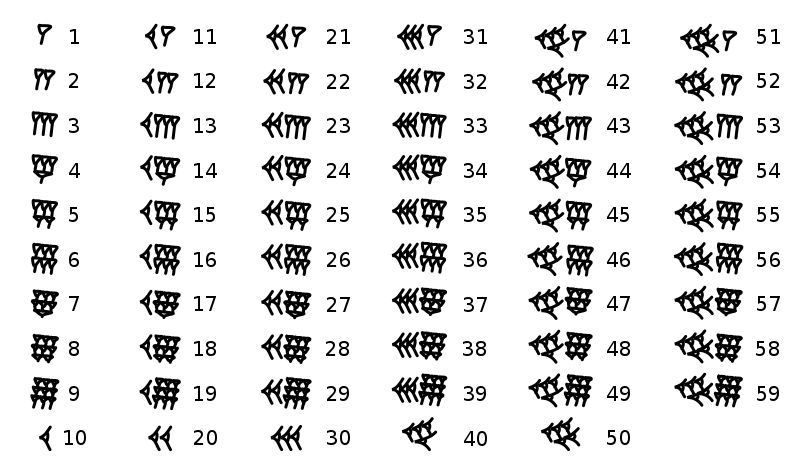
\includegraphics[width = 0.5 \textwidth]{media/babylonische_ziffern-320401102.png}
              \end{center}

              Unter den Keilschrift-Tafeln wurden einige gefunden, welche die Quadratzahlen
              \[
                  1,4,9,16,25,36,\ldots
              \]
              aufgelistet haben. Lange wurde darüber gerätselt, zu welchem Zweck diese Listen angefertigt wurden. Dann hat man herausgefunden, dass die Babylonier diese Listen dazu verwendeten, um beliebige Zahlen miteinander zu multiplizieren:

              Sollten die Zahlen \(a\) und \(b\) miteinander multipliziert werden, bildeten sie zunächst die Summe \((a+b)\) und die Differenz \((a-b)\), ermittelten dann die Quadrate der Summe und der Differenz mit Hilfe der Tafeln und subtrahierten anschliessend die beiden Zahlen voneinander. Schliesslich teilten sie das Ergebnis durch \(4\) und heraus kam das Produkt der beiden Zahlen \(a\) und \(b\).

              \begin{enumerate}
                  \item Berechnen Sie mit diesem Verfahren \(53\cdot47\).

                  \item Erstellen Sie einen Term für das Rechenverfahren der Babylonier und zeigen Sie, dass dieser Term tatsächlich gleich dem Produkt \(a\cdot b\) ist. (Nutzen Sie die binomischen Formeln.)

                  \item Welcher Zusammenhang besteht zwischen dem beschriebenen Rechenverfahren und der Grafik? Tipp: Berechnen Sie die Fläche des grossen Quadrates auf zwei Arten.

                        \begin{center}
                            \begin{tikzpicture}[scale=0.9]
                                % Äusseres Quadrat
                                \draw[thick] (0,0) rectangle (5,5);

                                % Innere Unterteilung
                                \draw[thick] (2,5) -- (2,2);
                                \draw[thick] (2,3) -- (5,3);
                                \draw[thick] (3,0) -- (3,3);
                                \draw[thick] (0,2) -- (3,2);

                                % Zentrales Quadrat
                                \fill[gray!35] (2,2) rectangle (3,3);
                                \draw[thick] (2,2) rectangle (3,3);

                                % Beschriftung oben
                                \node[above] at (1,5) {\(b\)};
                                \node[above] at (3.5,5) {\(a\)};

                                % Beschriftung rechts
                                \node[right] at (5,4) {\(b\)};
                                \node[right] at (5,1.5) {\(a\)};

                                % Beschriftung unten
                                \node[below] at (1.5,0) {\(a\)};
                                \node[below] at (4,0) {\(b\)};

                                % Beschriftung links
                                \node[left] at (0,3.5) {\(a\)};
                                \node[left] at (0,1) {\(b\)};
                            \end{tikzpicture}
                        \end{center}

                  \item Finden Sie eine andere Möglichkeit, wie man mit diesen Tafeln multiplizieren kann?
              \end{enumerate}
    \end{enumerate}
\end{LA}






\clearpage
\begin{satz}{Die Binomischen Formeln}{binomischeformeln}
    Für \(a,b\in\mathbb{R}\) gilt:
    \begin{enumerate}
        \item
              \[
                  (a+b)^2=a^2+2ab+b^2
              \]

        \item
              \[
                  (a-b)^2=a^2-2ab+b^2
              \]

        \item
              \[
                  (a+b)(a-b)=a^2-b^2
              \]
    \end{enumerate}
\end{satz}

\textbf{Beweis:}
Zum Beweis muss man bloss die linke Seite ausmultiplizieren. Für die erste Binomische Formel sähe das so aus:
\[
    (a+b)^2
    =(a+b)(a+b)
    =a^2+ab+ba+b^2
    =a^2+2ab+b^2.
\]
Die anderen Formeln können genau gleich bewiesen werden.

\begin{bsp}{Binomische Formeln}{binomischeformeln-bsp}
    Berechnen Sie mithilfe der Binomischen Formeln.
    \begin{enumerate}
        \item \((x+2y)^2\)
              \vspace*{2cm}
        \item \((-p+q)^2\)
              \vspace*{2cm}
        \item \((x^3+y)^2\)
              \vspace*{2cm}
        \item \((-a-b)^2\)
              \vspace*{2cm}
    \end{enumerate}
\end{bsp}


\clearpage
\begin{ueb}
    {Binomische Formeln}{binome}
    \begin{enumerate}
        \item
              \begin{enumerate}
                  \item \((2a+5)^2\)
                  \item \((1-7u)^2\)
                  \item \(\left(\frac{1}{3}a+b\right)^2\)
                  \item \((2n-m)(2n+m)\)
                  \item \((x^2+2)^2\)
                  \item \((4a-5b)^2\)
                  \item \(\left(\frac{1}{4}d-\frac{c}{2}\right)^2\)
                  \item \(\left(\frac{1}{2}x+y\right)\left(\frac{1}{2}x-y\right)\)
              \end{enumerate}

        \item
              \begin{enumerate}
                  \item \(\left(\frac{1}{a}-\frac{1}{b}\right)
                        \left(\frac{1}{b}+\frac{1}{a}\right)\)
                  \item \(\left(\frac{3}{4}a-1\right)^2\)
                  \item \((4x^2+9y^2)^2\)
                  \item \((x^2-1)(x^2+1)\)
                  \item \((-5y+x)^2\)
                  \item \((-x-y)(x+y)\)
                  \item \((-x-y)(x-y)\)
                  \item \((-a-3b)^2\)
              \end{enumerate}
        \item
              \begin{enumerate}
                  \item \(\left(x+\frac{1}{2}\right)\left(\frac{1}{2}-x\right)\)
                  \item \((2e-3f)(3f+2e)\)
                  \item \(2n(7p-6q+1)\)
                  \item \(a(a^2-2b)^2\)
                  \item \((-1)\cdot(2x-3y^2+2xy)\)
                  \item \(2c(c-5)^2\)
              \end{enumerate}

        \item
              \begin{enumerate}
                  \item \((3-y)^2(3+y)^2\)
                  \item \((a+b)^2\cdot\frac{1}{b}\)
                  \item \(\frac{1}{2}x\cdot(y+4)^2\)
                  \item \(\bigl[(2a+b)(2a-b)\bigr]^2\)
                  \item \(\frac{1}{x}\cdot(x+x^2)^2\)
                  \item \((a+4)^2-(a-2)^2\)
                  \item \((2x-y)^2+(2x+y)^2\)
                  \item \((2y+2z)^2-2(y+z)^2\)
                  \item \((5u-1)^2-(5u-1)(5u+1)\)
              \end{enumerate}
    \end{enumerate}
\end{ueb}

\clearpage
\emph{Lösungen}
\begin{enumerate}
    \item
          \begin{enumerate}
              \item \(4a^2+20a+25\)
              \item \(49u^2-14u+1\)
              \item \(\dfrac{1}{9}a^2+\dfrac{2}{3}ab+b^2\)
              \item \(4n^2-m^2\)
              \item \(x^4+4x^2+4\)
              \item \(16a^2-40ab+25b^2\)
              \item \(\dfrac{1}{16}d^2-\dfrac{1}{4}cd+\dfrac{1}{4}c^2\)
              \item \(\dfrac{1}{4}x^2-y^2\)
          \end{enumerate}

    \item
          \begin{enumerate}
              \item \(\dfrac{1}{a^2}-\dfrac{1}{b^2}\)
              \item \(\dfrac{9}{16}a^2-\dfrac{3}{2}a+1\)
              \item \(16x^4+72x^2y^2+81y^4\)
              \item \(x^4-1\)
              \item \(x^2-10xy+25y^2\)
              \item \(-x^2-2xy-y^2\)
              \item \(-x^2+y^2\)
              \item \(a^2+6ab+9b^2\)
          \end{enumerate}

    \item
          \begin{enumerate}
              \item \(\dfrac{1}{4}-x^2\)
              \item \(4e^2-9f^2\)
              \item \(14np-12nq+2n\)
              \item \(a^5-4a^3b+4ab^2\)
              \item \(-2x+3y^2-2xy\)
              \item \(2c^3-20c^2+50c\)
          \end{enumerate}

    \item
          \begin{enumerate}
              \item \(y^4-18y^2+81\)
              \item \(\dfrac{a^2}{b}+2a+b\)
              \item \(\dfrac{1}{2}xy^2+4xy+8x\)
              \item \(16a^4-8a^2b^2+b^4\)
              \item \(x^3+2x^2+x\)
              \item \(12a+12\)
              \item \(8x^2+2y^2\)
              \item \(2y^2+4yz+2z^2\)
              \item \(2-10u\)
          \end{enumerate}
\end{enumerate}























\clearpage
\subsection{Das Pascalsche Dreieck}
\begin{LA}{Pascalsches Dreieck}{pascalschesdreieck}
    Zur Vereinfachung von Termen der Form \((a+b)^n\) kann man das sogenannte \textit{Pascalsche Dreieck} verwenden. In dieser Lernaufgabe werden Sie dieses Dreieck selbst entdecken und als Hilfsmittel zur Bestimmung höherer Potenzen anwenden.

    \begin{enumerate}
        \item Berechnen Sie die folgenden Potenzen:
              \begin{enumerate}
                  \item \((a+b)^1\)
                  \item \((a+b)^2\)
                  \item \((a+b)^3\)
                  \item \((a+b)^4\)
              \end{enumerate}

        \item Ergänzen Sie mit den Resultaten aus Aufgabe 1) das folgende Dreieck, indem Sie wie in den ersten beiden Zeilen vorgemacht, die fehlenden Koeffizienten einfügen.
              \[
                  \begin{aligned}
                      (a+b)^1 & = \phantom{a^4+4a^3+6a^2}{\color{red}1}\,a+{\color{red}1}\,b                              \\
                      (a+b)^2 & = \phantom{a^4+4a^3+}{\color{red}1}\,a^2+{\color{red}2}\,ab+{\color{red}1}\,b^2           \\
                      (a+b)^3 & = \phantom{a^4+4}a^3+\phantom{1}\quad a^2b+\phantom{1}\quad ab^2+\quad b^3                \\
                      (a+b)^4 & = \quad a^4+\phantom{1}\quad a^3b+\phantom{1}\quad a^2b^2+\phantom{1}\quad ab^3+\quad b^4
                  \end{aligned}
              \]

        \item Untersuchen Sie das Resultat aus Aufgabe 2 und erklären Sie, wie sich die Koeffizienten einer Zeile aus jenen der Zeile davor berechnen lassen. Wie müssten demnach die nächsten drei Zeilen lauten?
              \begin{enumerate}
                  \item \((a+b)^5\)
                  \item \((a+b)^6\)
                  \item \((a+b)^7\)
              \end{enumerate}

              Lassen Sie das Resultat von der Lehrperson kontrollieren.

        \item Berechnen Sie die folgenden Potenzen:
              \begin{enumerate}
                  \item \((a-b)^1\)
                  \item \((a-b)^2\)
                  \item \((a-b)^3\)
                  \item \((a-b)^4\)
              \end{enumerate}

        \item Ergänzen Sie mit den Resultaten aus Aufgabe 4) das folgende Dreieck, indem Sie wie in der ersten Zeile vorgemacht, die fehlenden Koeffizienten einfügen.
              \[
                  \begin{aligned}
                      (a-b)^1 & = \phantom{a^4+4a^3+6a^2}{\color{red}1}\,a-{\color{red}1}\,b                              \\
                      (a-b)^2 & = \phantom{a^4+4a^3+}{\color{red}1}\,a^2-{\color{red}2}\,ab+{\color{red}1}\,b^2           \\
                      (a-b)^3 & = \phantom{a^4+4}a^3-\phantom{1}\quad a^2b+\phantom{1}\quad ab^2-\quad b^3                \\
                      (a-b)^4 & = \quad a^4-\phantom{1}\quad a^3b+\phantom{1}\quad a^2b^2-\phantom{1}\quad ab^3+\quad b^4
                  \end{aligned}
              \]

        \item Untersuchen Sie, wie sich die Koeffizienten im Dreieck entwickeln, und finden Sie eine Regelmässigkeit. Bestimmen Sie anschliessend \textbf{nur mit Hilfe des Dreiecks}
              \begin{enumerate}
                  \item \((a-b)^5\)
                  \item \((a-b)^6\)
                  \item \((a-b)^7\)
              \end{enumerate}

              Lassen Sie das Resultat von der Lehrperson kontrollieren.
    \end{enumerate}
\end{LA}

\clearpage
Zur Vereinfachung von Termen der Form \((a+b)^n\) kann man das sogenannte
\textit{Pascalsche Dreieck} verwenden. Dieses Zahlendreieck ist nach dem
französischen Mathematiker Blaise Pascal (1623--1662) benannt\footnote{
    Dieses Zahlendreieck war aber schon früher bekannt. Entsprechend hat das
    Dreieck in anderen Ländern auch andere Namen -- jeder bezieht sich auf einen
    Mathematiker aus der entsprechenden Gegend! In Italien wird es
    Tartaglia-Dreieck genannt, in China nennt man es das Yang-Hui-Dreieck und im
    Iran spricht man vom Chayyam-Dreieck.}.

\begin{bsp}{Anwendung des Pascalschen Dreiecks}{pascalbeispiel1}
    Zur Vereinfachung von \((a+b)^6\) verwenden wir die sechste Zeile des
    Pascalschen Dreiecks:
    \vspace*{10 cm}
    % \[
    %     \begin{array}{ccccccccccccc}
    %           &   &   &   &    &    & 1                            \\
    %           &   &   &   &    & 1  &    & 1                       \\
    %           &   &   &   & 1  &    & 2  &    & 1                  \\
    %           &   &   & 1 &    & 3  &    & 3  &    & 1             \\
    %           &   & 1 &   & 4  &    & 6  &    & 4  &   & 1         \\
    %           & 1 &   & 5 &    & 10 &    & 10 &    & 5 &   & 1     \\
    %         1 &   & 6 &   & 15 &    & 20 &    & 15 &   & 6 &   & 1
    %     \end{array}
    % \]

    % Die Koeffizienten von \((a+b)^6\) sind also
    % \[
    %     1,\;6,\;15,\;20,\;15,\;6,\;1.
    % \]
    % Damit erhält man
    % \[
    %     (a+b)^6
    %     =
    %     a^6+6a^5b+15a^4b^2+20a^3b^3+15a^2b^4+6ab^5+b^6.
    % \]
\end{bsp}

\begin{bsp}{Ein zweites Beispiel}{pascalbeispiel2}

    \[
        (x^2-2y)^4
    \]

    \vspace*{5 cm}
    % Wie verwenden die Koeffizienten
    % \[
    %     1,\;4,\;6,\;4,\;1.
    % \]
    % Somit gilt
    % \[
    %     \begin{aligned}
    %         (x^2-2y)^4
    %          & =(x^2)^4
    %         +4(x^2)^3(-2y)
    %         +6(x^2)^2(-2y)^2
    %         +4x^2(-2y)^3
    %         +(-2y)^4                               \\
    %          & =x^8-8x^6y+24x^4y^2-32x^2y^3+16y^4.
    %     \end{aligned}
    % \]
\end{bsp}

\clearpage
\begin{ueb}
    {Pascalsches Dreieck}{pascalschesdreieck}
    \begin{enumerate}
        \item
              \begin{enumerate}
                  \item \((2a+b)^3\)
                  \item \((a-2b)^3\)
                  \item \((3c+1)^4\)
                  \item \((4-d)^4\)
              \end{enumerate}

        \item
              \begin{enumerate}
                  \item \((2p+q)^5\)
                  \item \((-r+10)^5\)
                  \item \(\left(s+\dfrac{1}{2}\right)^4\)
                  \item \(\left(t+\dfrac{1}{t}\right)^4\)
              \end{enumerate}

        \item
              \begin{enumerate}
                  \item \((2x+y)^3-(2x-y)^3\)
                  \item \(\left(z+\dfrac{1}{2}\right)^4-\left(z-\dfrac{1}{2}\right)^4\)
                  \item \(\left(z+\dfrac{1}{2}\right)^4+\left(z-\dfrac{1}{2}\right)^4\)
                  \item \(\left(u-\dfrac{1}{u}\right)^3-\left(u+\dfrac{1}{u}\right)^3\)
              \end{enumerate}

        \item
              \begin{enumerate}
                  \item \((m^2+m)^3\)
                  \item \((n^2+2n)^3\)
                  \item \((p^3-1)^3\)
                  \item \((1-q^4)^4\)
              \end{enumerate}

        \item \textbf{Challenge}
              \begin{enumerate}
                  \item Berechnen Sie mit dem Taschenrechner die Potenzen
                        \[
                            11^0,\;11^1,\;11^2,\;11^3,\;11^4
                            \quad\text{und}\quad 11^5.
                        \]
                        Erklären Sie das Resultat.

                  \item Berechnen Sie zeilenweise die Summe der Zahlen im
                        Pascalschen Dreieck. Erklären Sie das Resultat.
              \end{enumerate}
    \end{enumerate}
\end{ueb}

\clearpage
\emph{Lösungen}
\begin{enumerate}
    \item
          \begin{enumerate}
              \item \(8a^3+12a^2b+6ab^2+b^3\)
              \item \(a^3-6a^2b+12ab^2-8b^3\)
              \item \(81c^4+108c^3+54c^2+12c+1\)
              \item \(d^4-16d^3+96d^2-256d+256\)
          \end{enumerate}

    \item
          \begin{enumerate}
              \item \(32p^5+80p^4q+80p^3q^2+40p^2q^3+10pq^4+q^5\)
              \item \(-r^5+50r^4-1000r^3+10000r^2-50000r+100000\)
              \item \(s^4+2s^3+\dfrac{3}{2}s^2+\dfrac{1}{2}s+\dfrac{1}{16}\)
              \item \(t^4+4t^2+6+\dfrac{4}{t^2}+\dfrac{1}{t^4}\)
          \end{enumerate}

    \item
          \begin{enumerate}
              \item \(24x^2y+2y^3\)
              \item \(4z^3+z\)
              \item \(2z^4+3z^2+\dfrac{1}{8}\)
              \item \(-6u-\dfrac{2}{u^3}\)
          \end{enumerate}

    \item
          \begin{enumerate}
              \item \(m^6+3m^5+3m^4+m^3\)
              \item \(n^6+6n^5+12n^4+8n^3\)
              \item \(p^9-3p^6+3p^3-1\)
              \item \(q^{16}-4q^{12}+6q^8-4q^4+1\)
          \end{enumerate}
\end{enumerate}
































\clearpage
\subsection{Faktorzerlegung}
\begin{LA}
    {Einführungsaufgabe}{E in Faktorzerlegung}
    Betrachten Sie den Bruch
    \[
        \frac{x^2+2x-15}{x-3}.
    \]

    \begin{enumerate}
        \item Setzen Sie für \(x\) die Zahlen \(0\), \(1\), \(2\), \(5\), \(10\) und \(-2\) ein und berechnen Sie den Wert des Bruches.
              Die Resultate können Sie in die Tabelle eintragen:

              \[
                  \renewcommand{\arraystretch}{2}
                  \begin{array}{
                          |>{\centering\arraybackslash}m{1.5cm}
                          |*{6}{>{\centering\arraybackslash}m{1.5cm}|}
                      }
                      \hline
                      x            & 0 & 1 & 2 & 5 & 10 & \(-2\) \\ \hline
                      \text{Bruch} &   &   &   &   &    &        \\ \hline
                  \end{array}
              \]

        \item Was vermuten Sie: Welchen Wert wird der Bruch annehmen, wenn man für \(x\) die Zahl \(723\) einsetzt?

        \item \textbf{Challenge:} Können Sie Ihre Vermutung mit einer Termumformung beweisen?
    \end{enumerate}
\end{LA}

\clearpage

Bis anhin haben wir Terme vereinfacht, indem wir alle Multiplikationen ausgeführt haben, bis am Schluss eine Summe von Monomen übrigblieb.

\textbf{Beispiel:}
\[
    (x+5)(x-3)
    = x^2+5x-3x-15
    = x^2+2x-15
\]

Diese Art der Darstellung eines Polynoms als \textbf{Summe} ist oft hilfreich. Es gibt aber Situationen, in welchen es hilfreicher ist, Polynome als \textbf{Produkte} zu schreiben. So ist der Bruch
\[
    \frac{x^2+2x-15}{x-3}
\]
auf den ersten Blick ziemlich kompliziert. Wenn man das Polynom im Zähler als ein Produkt darstellt, kann man kürzen und der Bruch wird plötzlich viel einfacher:
\[
    \frac{x^2+2x-15}{x-3}
    =
    \frac{(x+5)(x-3)}{x-3}
    =
    x+5
\]

In diesem Kapitel geht es also darum, Polynome in Produkte zu verwandeln. Diese Umformung nennt man auch \emph{Faktorzerlegung}. Dabei werden die Polynome in Faktoren zerlegt, oder kurz \emph{faktorisiert}.

Übrigens gibt es eine zweite, ganz wichtige Anwendung der Faktorzerlegung. Die Gleichung
\[
    x^2+2x-15=0
\]
ist in dieser Form ganz schwierig zu lösen. Viel einfacher wird es, wenn man die linke Seite faktorisiert:
\[
    (x+5)(x-3)=0
\]

Wenn das Produkt von zwei Zahlen Null ist, muss einer der beiden Faktoren Null sein. Die Gleichung geht also genau dann auf, wenn \(x=-5\) oder \(x=3\) ist.

\bigskip

Im Folgenden lernen Sie die wichtigsten Techniken kennen, wie man eine Summe in ein Produkt umwandeln kann:
\textbf{Ausklammern}

Das Ausklammern ist die einfachste Art, einen Term in ein Produkt zu verwandeln.
Kommt bei einem Polynom in jedem Summanden der gleiche Faktor vor, so kann man
diesen ausklammern.

\begin{bsp}{}{}
    \[
        8a^2b + 12ab^2 =
    \]
    \vspace*{1cm}
\end{bsp}
\clearpage
\textbf{Binomische Formeln}

Eine andere Möglichkeit, ein Polynom in ein Produkt zu verwandeln, ergibt sich,
wenn man die binomischen Formeln gewissermassen «rückwärts» anwendet. Im
folgenden Beispiel werden wir die erste binomische Formel
\[
    (a+b)^2 = a^2 + 2ab + b^2
\]
verwenden, um ein Polynom zu faktorisieren.

\begin{bsp}{}{}
    \[
        x^2 + 6x + 9
    \]
    \vspace*{1cm}
\end{bsp}

\begin{bsp}{}{}
    \[
        4x^2-y^2
    \]
    \vspace*{1cm}
\end{bsp}

\begin{bsp}{}{}
    \[
        32z^2-16z+2
    \]
    \vspace*{1cm}
\end{bsp}

\textbf{Der Satz von Vieta}

Zum Schluss lernen wir noch eine dritte Technik zur Faktorzerlegung von Polynomen
kennen: Der Satz von Vieta (benannt nach dem französischen Mathematiker
François Viète, 1540--1603).

\begin{LA}
    {Des Satz von Vieta}{}


    \begin{enumerate}
        \item \textbf{(Im Plenum)} Vereinfachen Sie die Terme durch Ausmultiplizieren:
              \begin{enumerate}
                  \item \((x+2)(x-3)=\)    \vspace*{0.5cm}
                  \item \((x+4)(x-3)=\)    \vspace*{0.5cm}
                  \item \((x+7)(x-3)=\)    \vspace*{0.5cm}
                  \item \((x+100)(x-3)=\)    \vspace*{0.5cm}
                  \item \((x+a)(x-3)=\)    \vspace*{0.5cm}
              \end{enumerate}

              Die Hilfsvariable \(a\) im letzten Term nennt man einen
              \emph{Parameter}. Sie ist nicht die Hauptvariable im Term.
              Aber durch deren Verwendung können wir alle Polynome der Form
              \((x+\text{etwas})(x-3)\) gleichzeitig untersuchen.

        \item \textbf{(Jeder für sich)} Vereinfachen Sie die Terme durch
              Ausmultiplizieren, finden Sie das «Muster».
              \begin{enumerate}
                  \item \((x+3)(x+4)=\)     \vspace*{0.5cm}
                  \item \((x+5)(x+1)=\)    \vspace*{0.5cm}
                  \item \((x+7)(x+2)=\)    \vspace*{0.5cm}
                  \item \((x+4)(x+9)=\)    \vspace*{0.5cm}
                  \item \((x+2)(x+(-3))=\)    \vspace*{0.5cm}
                  \item \((x+a)(x+b)=\)    \vspace*{0.5cm}
              \end{enumerate}

        \item \textbf{(Jeder für sich)} Faktorisieren Sie die Polynome.
              \begin{enumerate}
                  \item \(x^2+3x+2\)    \vspace*{0.5cm}
                  \item \(x^2+5x+6\)    \vspace*{0.5cm}
                  \item \(x^2+16x+63\)    \vspace*{0.5cm}
                  \item \(x^2-7x+10\)    \vspace*{0.5cm}
              \end{enumerate}
    \end{enumerate}
\end{LA}

\clearpage

\begin{bsp}
    {}{}
    \( q^2 -16q -36\)
    \vspace*{0.5cm}
\end{bsp}

\begin{bsp}
    {}{}
    \( b^2 +5b -24\)
    \vspace*{0.5cm}
\end{bsp}


\begin{bsp}
    {}{}
    \( 5a^2+10ab+5b^2\)
    \vspace*{0.5cm}
\end{bsp}


\begin{bsp}
    {}{}
    \( x^4-y^4\)
    \vspace*{0.5cm}
\end{bsp}


\begin{bsp}
    {}{}
    \( x^2(y-5)+x(5-y)-2(y-5)\)
    \vspace*{2cm}
\end{bsp}

\clearpage
\begin{ueb}
    {Faktorzerlegung}{}
    \emph{Ausklammern}
    \begin{enumerate}
        \item
              \begin{enumerate}
                  \item \(24z^3-16z^2\)
                  \item \(20y^2+12y\)
                  \item \(z^2-z\)
                  \item \(81y^3+54y\)
                  \item \(-15x+27y-12z\)
                  \item \(-14np-12nq-21n\)
              \end{enumerate}

        \item
              \begin{enumerate}
                  \item \(20ab-20a^2b+5ab^3\)
                  \item \(6x^2y^2-3xy^2+9x^2y\)
                  \item \(42m^3n^2-70m^2n^3-42m^2n^2\)
                  \item \(3qr^2+3r^3+3r^2s-r^2\)
              \end{enumerate}
    \end{enumerate}
    \emph{Binomische Formeln}
    \begin{enumerate}[resume]
        \item
              \begin{enumerate}
                  \item \(49a^2-36b^2\)
                  \item \(x^2+8x+16\)
                  \item \(100-x^2\)
                  \item \(25y^2-30xy+9x^2\)
                  \item \(9x^2-(2y)^2\)
                  \item \(16x^2-1\)
                  \item \(x^4-y^4\)
                  \item \(4f^2-20fg+25g^2\)
              \end{enumerate}

        \item
              \begin{enumerate}
                  \item \(16r^2-24rs+9s^2\)
                  \item \(p^4-8p^2+16\)
                  \item \(-9a^2+81b^2\)
                  \item \(2-50z^2\)
                  \item \(5a^2-10ab+5b^2\)
                  \item \(4c^2-c^2d^4\)
                  \item \(n^3-n\)
                  \item \(-18u^2+12uv-2v^2\)
              \end{enumerate}

        \item Setzen Sie für \(\square\), \(\bigcirc\) und \(\diamond\) einen passenden Term ein, sodass eine binomische Formel anwendbar wird. Schreiben Sie den Term anschliessend als Produkt.

              \begin{enumerate}
                  \item \(x^2-\square\cdot x+64\)
                  \item \(9x^2+\square+49\)
                  \item \(x^2+3x+\bigcirc\)
                  \item \(\diamond+2a^2b+\square\)
              \end{enumerate}

        \item
              \begin{enumerate}
                  \item \(-p^2+169\)
                  \item \(126a^2b+96ab^2\)
                  \item \(25x^4-80x^3+64x^2\)
                  \item \(18a^2b+18ab^2-9ab\)
                  \item \(18z^2-2\)
                  \item \(81u^2+9z^2\)
              \end{enumerate}

        \item
              \begin{enumerate}
                  \item \(8u^2+2z^2+8uz\)
                  \item \(x^2y^2-2xy+y^2\)
                  \item \(\dfrac{1}{4}a^2+ab+b^2\)
                  \item \(9a^2+6a+1\)
                  \item \(\dfrac{1}{9}x^4+2x^3+9x^2\)
                  \item \(-3u^2+18uv-27v^2\)
              \end{enumerate}

    \end{enumerate}
    \emph{Vieta}
    \begin{enumerate}[resume]
        \item
              \begin{enumerate}
                  \item \(x^2+9x+20\)
                  \item \(d^2+20d+91\)
                  \item \(r^2-15r+54\)
                  \item \(n^2-26n+144\)
                  \item \(n^2-24n+144\)
                  \item \(q^2-16q-36\)
                  \item \(s^2+18s+72\)
                  \item \(z^2-19z+48\)
                  \item \(p^2+23p+132\)
              \end{enumerate}

        \item
              \begin{enumerate}
                  \item \(y^2-29y+210\)
                  \item \(b^2+10b+9\)
                        %   \item \(a^2+6a-10\)
                  \item \(a^2+2a-24\)
                  \item \(u^2-3u-40\)
                  \item \(t^2-6t-7\)
                  \item \(x^2-25x+84\)
                  \item \(x^2+25x-84\)
                  \item \(m^2-m-110\)
              \end{enumerate}

        \item
              \begin{enumerate}
                  \item \(3c^2-9c-324\)
                  \item \(m^4+4m^2-5\)
                  \item \(-y^2+y+30\)
                  \item \(x^2z^2+9x^2z-90x^2\)
                  \item \(r^6-43r^3-240\)
                        %   \item \(y^2+40y+400\)
                        %   \item \(b^2+20b+51\)
                        %   \item \(t^2+t-156\)
                        %   \item \(x^2-4x+16\)
              \end{enumerate}

        \item Challenge
              \begin{enumerate}
                  \item \(3c^2+16c+5\)
                  \item \(2x^2-5x+2\)
                  \item \(4e^2+3e-1\)
                  \item \(5k^2-2k-3\)
                  \item \(2n^2+7n+3\)
                  \item \(12r^2-8r+1\)
              \end{enumerate}
    \end{enumerate}
\end{ueb}
\clearpage
\emph{Lösungen}
\begin{enumerate}
    \item
          \begin{enumerate}
              \item \(8z^2(3z-2)\)
              \item \(4y(5y+3)\)
              \item \(z(z-1)\)
              \item \(27y(3y^2+2)\)
              \item \(-3(5x-9y+4z)\)
              \item \(-n(14p+12q+21)\)
          \end{enumerate}

    \item
          \begin{enumerate}
              \item \(5ab(4-4a+b^2)\)
              \item \(3xy(2xy-y+3x)\)
              \item \(14m^2n^2(3m-5n-3)\)
              \item \(r^2(3q+3r+3s-1)\)
          \end{enumerate}

    \item
          \begin{enumerate}
              \item \((7a-6b)(7a+6b)\)
              \item \((x+4)^2\)
              \item \((10-x)(10+x)\)
              \item \((5y-3x)^2\)
              \item \((3x-2y)(3x+2y)\)
              \item \((4x-1)(4x+1)\)
              \item \((x-y)(x+y)(x^2+y^2)\)
              \item \((2f-5g)^2\)
          \end{enumerate}

    \item
          \begin{enumerate}
              \item \((4r-3s)^2\)
              \item \((p^2-4)^2=(p-2)^2(p+2)^2\)
              \item \(9(3b-a)(3b+a)\)
              \item \(2(1-5z)(1+5z)\)
              \item \(5(a-b)^2\)
              \item \(c^2(2-d^2)(2+d^2)\)
              \item \(n(n-1)(n+1)\)
              \item \(-2(3u-v)^2\)
          \end{enumerate}

    \item
          \begin{enumerate}
              \item \(\square=16,\qquad x^2-16x+64=(x-8)^2\)
              \item \(\square=42x,\qquad 9x^2+42x+49=(3x+7)^2\)
              \item \(\bigcirc=\dfrac94,\qquad x^2+3x+\dfrac94=\left(x+\dfrac32\right)^2\)
              \item \(\diamond=a^4,\quad \square=b^2,\qquad
                    a^4+2a^2b+b^2=(a^2+b)^2\)
          \end{enumerate}

    \item
          \begin{enumerate}
              \item \((13-p)(13+p)\)
              \item \(6ab(21a+16b)\)
              \item \(x^2(5x-8)^2\)
              \item \(9ab(2a+2b-1)\)
              \item \(2(3z-1)(3z+1)\)
              \item \(9(9u^2+z^2)\)
          \end{enumerate}

    \item
          \begin{enumerate}
              \item \(2(2u+z)^2\)
              \item \(y(x^2y-2x+y)\)
              \item \(\dfrac14(a+2b)^2\)
              \item \((3a+1)^2\)
              \item \(\dfrac19x^2(x+9)^2\)
              \item \(-3(u-3v)^2\)
          \end{enumerate}

    \item
          \begin{enumerate}
              \item \((x+4)(x+5)\)
              \item \((d+7)(d+13)\)
              \item \((r-9)(r-6)\)
              \item \((n-18)(n-8)\)
              \item \((n-12)^2\)
              \item \((q-18)(q+2)\)
              \item \((s+6)(s+12)\)
              \item \((z-16)(z-3)\)
              \item \((p+11)(p+12)\)
          \end{enumerate}

    \item
          \begin{enumerate}
              \item \((y-15)(y-14)\)
              \item \((b+1)(b+9)\)
                    %   \item \((a+3-\sqrt{19})(a+3+\sqrt{19})\)
              \item \((a-4)(a+6)\)
              \item \((u-8)(u+5)\)
              \item \((t-7)(t+1)\)
              \item \((x-21)(x-4)\)
              \item \((x-3)(x+28)\)
              \item \((m-11)(m+10)\)
          \end{enumerate}

    \item
          \begin{enumerate}
              \item \(3(c-12)(c+9)\)
              \item \((m-1)(m+1)(m^2+5)\)
              \item \((6-y)(y+5) = -(y-6)(y+5)\)
              \item \(x^2(z-6)(z+15)\)
              \item \((r^3-48)(r^3+5)\)
                    %   \item \((y+20)^2\)
                    %   \item \((b+3)(b+17)\)
                    %   \item \((t-12)(t+13)\)
                    %       \item nicht über \(\mathbb{R}\) in Linearfaktoren zerlegbar
          \end{enumerate}

    \item
          \begin{enumerate}
              \item \((3c+1)(c+5)\)
              \item \((2x-1)(x-2)\)
              \item \((4e-1)(e+1)\)
              \item \((5k+3)(k-1)\)
              \item \((2n+1)(n+3)\)
              \item \((6r-1)(2r-1)\)
          \end{enumerate}
\end{enumerate}



\clearpage
\textbf{Zusatz: Faktorzerlegung bei Zahlen -- Primzahlen}

\begin{definition}{Primzahl}{primzahl}
    Eine Zahl heisst \textit{Primzahl}, wenn sie genau zwei Teiler besitzt.
\end{definition}

\textbf{Bemerkung:} Die Zahl \(1\) hat genau einen Teiler (nämlich \(1\)). Also ist \(1\) keine Primzahl.

\begin{satz}{Fundamentalsatz der Zahlentheorie}{fundamentalsatzzahlentheorie}
    Jede natürliche Zahl \(n>1\) lässt sich eindeutig als Produkt der Form
    \[
        n=p_1^{e_1}\cdot p_2^{e_2}\cdot\ldots\cdot p_k^{e_k}
    \]
    schreiben, wobei \(p_1,p_2,\ldots,p_k\) Primzahlen und
    \(e_1,e_2,\ldots,e_k\) natürliche Zahlen sind.
\end{satz}

\textbf{Beispiel:}
\[
    360=2^3\cdot3^2\cdot5
\]

\begin{satz}{Unendlich viele Primzahlen}{unendlichvieleprimzahlen}
    Es gibt unendlich viele Primzahlen.
\end{satz}

\textbf{Beweis:}

\clearpage

\textbf{Grosse Primzahlen}

Die grösste bekannte Primzahl wurde im Jahr 2024 entdeckt. Sie lautet
\[
    2^{136279841}-1
\]
und ist \(41'024'320\) Dezimalstellen lang!

Einige ähnliche Zahlen lassen sich aber sofort ausschliessen:

\begin{enumerate}
    \item Wieso ist \(2^{2026}+4\) keine Primzahl?
    \item Wieso ist \(3^{2026}-15\) keine Primzahl?
    \item Wie kann man ausschliessen, dass \(2^{2026}-1\) eine Primzahl ist?
          (Denken Sie an die binomischen Formeln \ldots)
    \item Und nun noch einige Herausforderungen. Zeigen Sie, dass die folgenden Zahlen nicht prim sind:
          \begin{enumerate}
              \item \(2^{2026}+2^{1014}+1\)
              \item \(2^{2026}+2^{1015}-5\)
          \end{enumerate}
\end{enumerate}

\textbf{Einige offene Fragen rund um Primzahlen}

\begin{itemize}
    \item Gibt es unendlich viele Primzahlzwillinge -- also solche, die sich nur um \(2\) unterscheiden wie \(3\) und \(5\), \(11\) und \(13\), \(149\) und \(151\)? (Im Jahr 2013 ist dazu ein wichtiger Schritt gelungen. Vielleicht kann die Vermutung schon bald bewiesen werden.)

    \item Lässt sich jede gerade natürliche Zahl grösser als \(4\) als Summe zweier Primzahlen schreiben?
\end{itemize}




























\clearpage
\subsection{Lineare Gleichungen}
\begin{LA}
    {Einführung}{E in linGl}
    \begin{enumerate}
        \item Lösen Sie die Gleichungen:
              \begin{enumerate}
                  \item \(3x=15\)\vspace{2cm}
                  \item \(2x-6=0\)\vspace{2cm}
                  \item \(2(x+1)-5=7-3x\) \vspace{4cm}
                  \item \((x+1)^2+2=(x-2)^2-7\)
              \end{enumerate}
              \clearpage
        \item Schreiben Sie eine Anweisung aus höchstens vier Teilschritten, mit der man Gleichungen wie jene von Aufgabe 1) lösen kann.

              \begin{enumerate}
                  \item[1. Schritt:] \vspace{1.2cm}
                  \item[2. Schritt:] \vspace{1.2cm}
                  \item[3. Schritt:] \vspace{1.2cm}
                  \item[4. Schritt:] \vspace{1.2cm}
              \end{enumerate}
              \vspace{1.2cm}
        \item Anna möchte in der Mathematik unbedingt eine 5 im Zeugnis erreichen. In den bisherigen drei Prüfungen hat sie die folgenden Resultate erzielt:
              \begin{itemize}
                  \item 1. Prüfung: \(4.75\)
                  \item 2. Prüfung: \(5\)
                  \item 3. Prüfung: \(5.25\)
              \end{itemize}

              Zudem hat sie eine \(5\) als Mündlichnote, welche aber nur halb so viel zählt wie eine Prüfung.

              Nun möchte sie wissen, welche Note sie in der vierten und letzten Prüfung mindestens erzielen muss, damit ihr Notendurchschnitt \(4.75\) beträgt (und sie damit eine \(5\) im Zeugnis erhält).

              \begin{enumerate}
                  \item Stellen Sie eine Gleichung für dieses Problem auf.
                  \item Lösen Sie die Gleichung nach Ihrer Anweisung aus Aufgabe 2).
              \end{enumerate}
    \end{enumerate}
\end{LA}
\clearpage
Viele Fragen aus den verschiedensten Wissenschaften werden mit mathematischen Mitteln angegangen. Häufig läuft es darauf hinaus, dass eine Gleichung gelöst werden muss. In diesem Kapitel werden wir zunächst die einfachste Art von Gleichungen untersuchen: die sogenannten \textit{linearen Gleichungen}.

\begin{definition}{Lineare Gleichung}{linearegleichung}
    Eine Gleichung heisst linear, wenn sie sich auf die Form
    \[
        ax+b=0
    \]
    bringen lässt, wobei \(a\) und \(b\) zwei beliebige reelle Zahlen sind und \(x\) die Unbekannte bezeichnet.
\end{definition}

\begin{bsp}{Lineare Gleichungen}{}
    \begin{enumerate}
        \item Die Gleichung \(2x-5=0\) ist linear, weil sie die Form \(ax+b=0\) hat für \(a=2\) und \(b=-5\).

        \item Die Gleichung \(2x+3=x\) ist auch linear, denn sie kann zu \(x+3=0\) umgeformt werden und hat somit die Form \(ax+b=0\) für \(a=1\) und \(b=3\).

        \item Weitere Beispiele:

              \begin{center}
                  \renewcommand{\arraystretch}{1.8}
                  \begin{tabular}{|>{\centering\arraybackslash}p{0.44\textwidth}|>{\centering\arraybackslash}p{0.44\textwidth}|}
                      \hline
                      \textbf{Lineare Gleichungen} & \textbf{Nicht-lineare Gleichungen}      \\
                      \hline
                      \(2x+5=0\)                   & \(x^2+8x+6=0\)                          \\
                      \hline
                      \(23(x-1)=7(x+2)\)           & \(\displaystyle\frac{1}{\sqrt{x+1}}=2\) \\
                      \hline
                      \(x^2+7x-2=x^2\)             & \(3^x=100\)                             \\
                      \hline
                  \end{tabular}
              \end{center}
    \end{enumerate}
\end{bsp}

Im Beispiel 2 wurde eine Gleichung bereits umgeformt. Dabei stellt sich die Frage, welche Umformungen überhaupt zulässig sind. Nun: Eine Umformung ist dann zulässig, wenn die neu entstandene Gleichung dieselben Lösungen besitzt wie die ursprüngliche. Genauer:

\begin{definition}{Lösungsmenge und äquivalente Gleichungen}{loesungsmenge}
    Die Menge aller Zahlen, welche eine gegebene Gleichung lösen, heisst die \textit{Lösungsmenge} \(\mathbb{L}\) der Gleichung.

    Zwei Gleichungen heissen \textit{äquivalent}, wenn sie dieselbe Lösungsmenge haben.
\end{definition}

Jene Umformungen, welche die Lösungsmenge von Gleichungen nicht verändern, heissen \textit{Äquivalenzumformungen}. Davon gibt es im Wesentlichen zwei:
\begin{satz}{Äquivalenzumformungen}{aequivalenzumformungen}

    \begin{itemize}
        \item Auf beiden Seiten der Gleichung dieselbe Zahl addieren oder subtrahieren.
        \item Auf beiden Seiten der Gleichung mit derselben, von Null verschiedenen Zahl multiplizieren oder dividieren.
    \end{itemize}
\end{satz}

Gleichungen werden nun so gelöst, dass man sie so lange unter Anwendung von Äquivalenzumformungen verändert, bis die Lösung gewissermassen auf der Hand liegt. Zur Übersicht schreibt man neben der Gleichung hin, welche Umformung jeweils verwendet wird:

\begin{bsp}{Lösen einer linearen Gleichung}{}
    \[
        7x+4=2x-8
    \]

    \vspace{3cm}

    Die Lösungsmenge
    \[
        \mathbb{L}=\left\{\hspace{1.5cm}\right\}
    \]
    kann nun von der letzten Gleichung direkt abgelesen werden.
\end{bsp}

\subsection*{Sonderfälle}

Von einem Sonderfall ist die Rede, wenn beim Lösen der Gleichung die Unbekannte ``rausfällt''. Dabei entstehen zwei mögliche Situationen, die im Folgenden an Beispielen gezeigt werden:

\begin{enumerate}
    \item \textbf{Möglichkeit:}
          \[
              4(x+1)=4x+3
          \]

          \vspace{3cm}

    \item \textbf{Möglichkeit:}
          \[
              3(3-x)=-2x-(x-9)
          \]

          \vspace{3cm}
\end{enumerate}

\subsubsection*{Produkt = Null}

Eine spezielle Art von Gleichung sind solche, bei denen ein Produkt von zwei Termen Null ergibt, zum Beispiel:
\[
    (3x+1)(x-4)=0
\]

Wenn man die linke Seite der Gleichung ausmultipliziert, erhält man
\[
    3x^2-11x-4=0.
\]
Das ist keine lineare Gleichung (sondern eine quadratische, siehe später) und in der ausmultiplizierten Form nicht einfach zu lösen!

Betrachten wir aber die ursprüngliche, faktorisierte Form, so lässt sich die Lösungsmenge leicht bestimmen. Das Produkt
\[
    (3x+1)(x-4)
\]
kann nur dann Null ergeben, wenn einer der beiden Faktoren Null ist. Also muss
\[
    (3x+1)=0
\]
oder
\[
    (x-4)=0
\]
sein. Aus der quadratischen Gleichung sind so zwei lineare Gleichungen entstanden, die leicht zu lösen sind:
\[
    3x+1=0
    \quad\Longleftrightarrow\quad
    x=-\frac13
\]
und
\[
    x-4=0
    \quad\Longleftrightarrow\quad
    x=4.
\]

Die Gleichung hat zwei Lösungen:
\[
    \mathbb{L}=\left\{-\frac13,4\right\}.
\]

\clearpage
\begin{ueb}
    {Zu Produkt = 0 und lineare Gleichungen}{}
    \begin{enumerate}

        \item Bestimmen Sie die Lösung der Gleichung.

              \begin{enumerate}
                  \item \((x+3)^2-(2x-1)^2=(3+x)(x-3)-4x^2-13\)

                  \item \(2\cdot\bigl[3-4\cdot(x+2)-2\bigr]
                        +\dfrac{1}{2}\cdot\bigl[2-4\cdot(x-1)\bigr]=0\)

                  \item \((8x-1)(x+3)=8(x-2)^2\)

                  \item \(3\cdot(4x-2)+(1-x)^2
                        =\left(x+\dfrac{1}{3}\right)^2+3\cdot(2-3x)\)
                  \item \((x+2)^2-(x-3)^2=10x-4\)
                  \item \((x+4)(x-2)-(x+1)^2=-9\)
              \end{enumerate}
        \item Produkt = 0
              \begin{enumerate}
                  \item \((x+3)(2x-1)=0\)
                  \item \(x(2x+2)=0\)
                  \item \(3x^2-2x=0\)
                  \item \(x^2+2x+1=0\)
                  \item \(x^2-3x-28=0\)
                  \item \(2x^2+10x+12=0\)
              \end{enumerate}
        \item Berechnen Sie die Lösung der Gleichung im Kopf.

              \begin{enumerate}
                  \item \(6\cdot(3x+1)=100-4\cdot(3x+1)\)
                  \item \(x+321=456+320\)
                  \item \(0.7\cdot(8x+1)=50-1.3\cdot(8x+1)\)
                  \item \(314x+123x=246+314x\)
                  \item \(21x+35=7\cdot(9-x)\)
                  \item \(5x-x(x-3)=4+x-x(x-3)\)
              \end{enumerate}
    \end{enumerate}
\end{ueb}
\clearpage
\emph{Lösungen:}
\begin{enumerate}
    \item
          \begin{enumerate}
              \item \(\mathbb{L}=\{-3\}\)
              \item \(\mathbb{L}=\left\{-\dfrac{11}{10}\right\}\)
              \item \(\mathbb{L}=\left\{\dfrac{7}{11}\right\}\)
              \item \(\mathbb{L}=\left\{\dfrac{20}{33}\right\}\)
              \item \(\mathbb{L}=\emptyset\)
              \item \(\mathbb{L}=\R\)
          \end{enumerate}

    \item
          \begin{enumerate}
              \item \(\mathbb{L}=\left\{-3,\dfrac{1}{2}\right\}\)
              \item \(\mathbb{L}=\{-1,0\}\)
              \item \(\mathbb{L}=\left\{0,\dfrac{2}{3}\right\}\)
              \item \(\mathbb{L}=\{-1\}\)
              \item \(\mathbb{L}=\{-4,7\}\)
              \item \(\mathbb{L}=\{-3,-2\}\)
          \end{enumerate}

    \item
          \begin{enumerate}
              \item \(\mathbb{L}=\{3\}\)
              \item \(\mathbb{L}=\{455\}\)
              \item \(\mathbb{L}=\{3\}\)
              \item \(\mathbb{L}=\{2\}\)
              \item \(\mathbb{L}=\{1\}\)
              \item \(\mathbb{L}=\{1\}\)
          \end{enumerate}
\end{enumerate}
















\clearpage
\subsubsection*{Der Kleine Gauss}
Carl Friedrich Gauss (1777--1855) war ein deutscher Mathematiker und Astronom\footnote{Gauss liebte die reine Mathematik mehr als ihre Anwendungen. So soll er einmal gesagt haben:
    ``Ob ich die Mathematik auf ein paar Dreckklumpen anwende, die wir Planeten nennen, oder auf rein
    arithmetische Probleme, es bleibt sich gleich, die letzteren haben nur noch einen höheren Reiz für mich.''}
Durch seine Werke wurde er zu einem der wichtigsten Mathematiker, die je gelebt haben.
Laut einer Legende war sein mathematisches Talent schon in sehr jungen Jahren stark ausgeprägt:

Als Gauss neun Jahre alt war, stellte sein Lehrer der Klasse einen besonders schwierigen Auftrag:
Was erhält man, wenn man die ersten 100 Zahlen addiert? Oder anders gesagt: Was ist das Resultat der Rechnung
\[
    1+2+3+4+\dots+97+98+99+100\,?
\]

Der Lehrer meinte, die Schüler damit für den Rest der Stunde zu beschäftigen, aber Carl Friedrich Gauss
hatte das Resultat bereits nach wenigen Minuten. Schauen wir uns an, wie er das gemacht hat:

\begin{LA}
    {Kleiner Gauss}{KleinerGauss}

    \[
        1+2+3+\dots+48+49+50+51+52+53+\dots+98+99+100
    \]
    \vspace*{5cm}
    \begin{enumerate}
        \item Klammern
              \begin{enumerate}
                  \item Verbinden Sie auch 2 und 99 mit einer Klammer. Dann 3 und 98 und so weiter.
                  \item Wie gross ist die Summe der ersten 100 Zahlen?
              \end{enumerate}

        \item Verwenden Sie den ``Gauss-Trick'' für die folgende Summe:
              \[
                  1+2+\dots+499+500
              \]

        \item Wie lautet eine Formel für die Summe
              \[
                  1+2+3+\dots+n,
              \]
              falls \(n\) eine gerade Zahl ist?

        \item Der ``Gauss-Trick'' funktioniert für die Summe
              \[
                  1+2+\dots+776+777
              \]
              nicht ohne Weiteres. Was läuft schief, wenn die letzte Zahl ungerade ist?
              Wie kann man die Methode für diesen Fall anpassen?
              Was ergibt dann die Summe?

        \item Wie lautet eine Formel für die Summe
              \[
                  1+2+3+\dots+n,
              \]
              falls \(n\) eine ungerade Zahl ist?

        \item Wie berechnen Sie
              \[
                  64+65+66+\dots+123+124+125\,?
              \]

    \end{enumerate}
\end{LA}


\clearpage
\begin{satz}{Der ``kleine Gauss''}{kleinergauss}
    Für die Summe der ersten \(n\) natürlichen Zahlen gilt
    \[
        1+2+3+\dots+n=\qquad.
    \]
\end{satz}

Diese Summenformel kommt manchmal unerwartet zur Anwendung. Betrachten Sie dazu das folgende Beispiel.

\begin{bsp}{Silvesterparty}{silvesterparty}
    An einer Silvesterparty stösst jeder Gast mit jedem Gast einmal an. Wie oft klingen die Gläser, wenn 20 Gäste anwesend sind?

    \textbf{Antwort:} Wir stellen uns vor, dass die Gäste nacheinander zur Feier erscheinen und beim Eintreffen mit allen bereits Anwesenden anstossen:
    \begin{itemize}
        \item Die erste Person stösst beim Eintreffen mit niemandem an.
        \item Die zweite Person stösst mit der ersten an, also einmal.
        \item Die dritte Person stösst mit den beiden ersten an, also zweimal.
        \item \(\dots\)
        \item Die zwanzigste und letzte Person stösst mit den bereits Anwesenden an, also 19 Mal.
    \end{itemize}

    Insgesamt erklingen die Gläser also \(0+1+2+\dots+19\) Mal. Mit dem kleinen Gauss für \(n=19\) folgt
    \[
        0+1+2+\dots+19
        =\qquad
    \]


\end{bsp}

\begin{ueb}{Silvesterparty}{}
    An einer Silvesterparty stösst jeder Gast mit jedem Gast einmal an. Insgesamt erklingen die Gläser 78 Mal. Wie viele Gäste sind anwesend?

    \emph{Hinweis:} Man kann dieses Problem natürlich durch Ausprobieren lösen. Lehrreicher ist es aber, wenn man es mit einer Gleichung versucht. Diese lässt sich mit der Methode \enquote{Produkt = 0} lösen\dots
\end{ueb}

\begin{ueb}{CHALLENGE: Diagonalen eines Vielecks}{}
    Wie viele Ecken hat ein Vieleck mit 54 Diagonalen?
\end{ueb}


\emph{Lösungen:} 13 Gäste und 12 Ecken. Die wichtigere Frage ist aber, wie die entsprechenden Gleichungen lauten und wie man diese löst\dots





\pagebreak
\subsection{Lineare Gleichungen mit Parametern}
\begin{LA}
    {Einführung}{}
    \begin{center}
        \begin{tikzpicture}[scale=1.1]
            % Vorderseite
            \coordinate (A) at (0,0);
            \coordinate (B) at (4,0);
            \coordinate (C) at (4,2);
            \coordinate (D) at (0,2);

            % Rückseite
            \coordinate (E) at (1.2,0.8);
            \coordinate (F) at (5.2,0.8);
            \coordinate (G) at (5.2,2.8);
            \coordinate (H) at (1.2,2.8);

            % Vorderseite
            \draw (A) -- node[midway,below] {\(a\)} (B)
            -- (C)
            -- (D)
            -- cycle;

            % Verbindung zur Rückseite
            \draw (A) -- (E);
            \draw (B) -- node[midway,below right] {\(b\)} (F);
            \draw (C) -- (G);
            \draw (D) -- (H);

            % Rückseite
            \draw (E) -- (F)
            -- node[midway,right] {\(c\)} (G)
            -- (H)
            -- cycle;
        \end{tikzpicture}
    \end{center}

    Die Oberfläche eines Quaders mit den Kanten \(a\), \(b\) und \(c\) kann man mit folgender Formel berechnen:
    \[
        A = 2(ab+ac+bc)
    \]

    \begin{enumerate}
        \item Berechnen Sie die Länge der Kante \(c\), falls
              \begin{enumerate}
                  \item \(A=76\,\mathrm{m}^2,\quad a=2\,\mathrm{m},\quad b=4\,\mathrm{m}\)
                  \item \(A=62\,\mathrm{m}^2,\quad a=3\,\mathrm{m},\quad b=7\,\mathrm{m}\)
                  \item \(A=38\,\mathrm{m}^2,\quad a=1\,\mathrm{m},\quad b=4\,\mathrm{m}\)
                  \item \(A=96\,\mathrm{m}^2,\quad a=4\,\mathrm{m},\quad b=4\,\mathrm{m}\)
              \end{enumerate}

        \item Geben Sie eine Formel an, mit der man die Länge der Kante \(c\) direkt aus der Fläche \(A\) und den Kanten \(a\) und \(b\) berechnen kann. Überprüfen Sie anschliessend die Resultate aus Aufgabe 1) mit der gefundenen Formel.
    \end{enumerate}
\end{LA}





\clearpage
Wir haben Parameter bereits einmal verwendet, als wir den Satz von Vieta besprochen haben. Damals haben wir Terme der Form
\[
    (x+2)(x+6)
\]
oder
\[
    (x+1)(x+3)
\]
ausmultipliziert. Damit wir diese Multiplikationen nicht jedes Mal von vorne ausführen mussten, haben wir die Parameter \(a\) und \(b\) eingeführt und eine Formel aufgestellt:
\[
    (x+a)(x+b)=x^2+(a+b)x+ab.
\]

Parameter dienen dazu, viele ähnliche Probleme auf einmal zu lösen. Genauso war es in der Einführungsaufgabe. In der ersten Aufgabe ist immer dasselbe gesucht: die Länge von \(c\). Es ändern sich nur die Werte von \(A\), \(a\) und \(b\). Man kann nun diese Aufgaben unabhängig voneinander lösen. Dazu muss man jedes Mal eine Gleichung lösen. Oder man löst die Gleichung nur einmal in allgemeiner Form auf:
\[
    A=2(ab+ac+bc).
\]

Da wir die Länge von \(c\) bestimmen möchten, ist \(c\) die Unbekannte und \(A\), \(a\) und \(b\) die Parameter.

\[
    \begin{aligned}
        A     & = 2(ab+ac+bc) &  & \mid \text{TU} \\
        A     & = 2ab+2ac+2bc &  & \mid -2ab      \\
        A-2ab & = 2ac+2bc
    \end{aligned}
\]

Nun ist die Unbekannte \(c\) rechts und alles andere links vom Gleichheitszeichen. Um zu verstehen, wie es nun weitergeht, überlegen wir uns kurz, wie diese Situation aussehen würde, wenn \(A\), \(a\) und \(b\) ganz konkrete Zahlen wären. Für \(A=76\), \(a=2\) und \(b=4\) zum Beispiel erhalten wir:
\[
    76-2\cdot2\cdot4=2\cdot2c+2\cdot4c.
\]

In diesem konkreten Fall stünde auf der rechten Seite insgesamt \(12c\) und wir würden die Gleichung durch \(12\) teilen, um das Resultat zu erhalten.

Jetzt blicken wir wieder auf unsere allgemeine Gleichung
\[
    A-2ab=2ac+2bc.
\]

Wie viel mal \(c\) steht eigentlich auf der rechten Seite? Das erkennt man, wenn man \(c\) \textbf{ausklammert}:
\[
    A-2ab=(2a+2b)c.
\]

Auf der rechten Seite kommt die Grösse \(c\) insgesamt \((2a+2b)\)-mal vor. Dividiert man nun die Gleichung durch \((2a+2b)\), erhält man die gesuchte Formel für \(c\):
\[
    c=\frac{A-2ab}{2a+2b}.
\]

\begin{satz}{Rezept zum Lösen von linearen Gleichungen mit Parametern}{}
    \begin{enumerate}
        \item Mit Termumformungen beide Seiten vereinfachen.
        \item Mit Äquivalenzumformungen die Unbekannte auf die eine Seite und alles andere auf die andere Seite bringen.
        \item \textbf{Die Unbekannte ausklammern.}
        \item Die Gleichung durch den Vorfaktor der Unbekannten teilen.
    \end{enumerate}
\end{satz}
\begin{bsp}{Lineare Gleichung mit Parametern}{}
    Gesucht ist \(x\):
    \[
        4-2(ax+b)=b(x-1)
    \]
    \vspace*{4cm}
\end{bsp}

In der Physik, in der Geometrie und in vielen anderen Anwendungsgebieten werden Grössen durch eine Gleichung in Verbindung gebracht. Je nachdem, welche dieser Grössen gesucht oder gegeben sind, muss man die Gleichung nach der einen oder anderen Variable auflösen.

\begin{bsp}{Flächeninhalt eines Trapezes}{}
    Die Fläche \(A\) eines Trapezes, dessen beiden Grundseiten \(a\) und \(c\) und dessen Höhe \(h\) sind, wird durch die Formel
    \[
        A=\frac{a+c}{2}\cdot h
    \]
    beschrieben.

    Diese Gleichung ist praktisch, wenn \(a\), \(c\) und \(h\) gegeben sind und \(A\) gesucht wird. Wenn hingegen \(h\) gesucht ist, sollte man die Gleichung nach \(h\) auflösen:
    \[
        A=\frac{a+c}{2}\cdot h
    \]

    \clearpage

    Wenn jedoch \(a\) gesucht wird, sollte man sie entsprechend nach \(a\) auflösen:
    \[
        A=\frac{a+c}{2}\cdot h
    \]

    \vspace{3cm}
\end{bsp}

\begin{ueb}
    {Lineare Gleichung mit Parametern}{}
    \begin{enumerate}
        \item Lösen Sie die Gleichung nach \(x\) auf. Bewahren Sie die Lösungen sicher auf, Sie werden sie in einer späteren Aufgabe wieder benötigen.

              \begin{enumerate}
                  \item \(cx+c=dx\)
                  \item \(ax=a^2+a\)
                  \item \(qx=1-px\)
                  \item \(qx=-px\)
                  \item \(ax-b=2b+x\)
                  \item \((a+b)x=a^2+2ab+b^2\)
                  \item \(x-p=p^2-px\)
                  \item \(q+3qx=x\)
              \end{enumerate}
    \end{enumerate}
\end{ueb}
\clearpage
\emph{Lösungen:}
\begin{enumerate}
    \item \(x=\dfrac{c}{d-c}\)
    \item \(x=a+1\)
    \item \(x=\dfrac{1}{p+q}\)
    \item \(x=0\)
    \item \(x=\dfrac{3b}{a-1}\)
    \item \(x=a+b\)
    \item \(x=p\)
    \item \(x=\dfrac{q}{1-3q}\)
\end{enumerate}










\clearpage
\subsection{Sonderfälle bei Gleichungen mit Parameter}
\begin{LA}
    {Das Oma-Problem}{Oma}
    Bobs Grossmutter ist \(d\) Jahre älter als seine Mutter. Bob behauptet: ``Wenn ich \(d\) Jahre alt bin, bin ich doppelt so alt wie meine Grossmutter!''

    Das mag seltsam klingen, aber Bob kann das sogar beweisen:

    Sei \(M\) das Alter von Bobs Mutter, \(G\) jenes von Bobs Grossmutter und \(d\) jenes von Bob.

    \textbf{Voraussetzung:}
    \[
        G-M=d
    \]
    oder umgestellt:
    \[
        G=M+d
        \qquad\text{beziehungsweise}\qquad
        M=G-d.
    \]

    \textbf{Behauptung:}
    \[
        d=2G.
    \]

    \textbf{Beweis:}
    Die Reihenfolge bei der Multiplikation spielt bekanntlich keine Rolle, also ist
    \[
        G\cdot M=M\cdot G.
    \]

    Nun verwenden wir auf der linken Seite die Voraussetzung \(M=G-d\) und rechts \(G=M+d\):
    \[
        \begin{aligned}
            G(G-d)    & = M(M+d)     &  & \mid -MG \\
            G(G-d)-MG & = M(M+d)-MG.
        \end{aligned}
    \]

    Auf der linken Seite können wir \(G\) ausklammern, rechts hingegen \(M\). Man erhält
    \[
        \begin{aligned}
            G(G-d-M) & = M(M+d-G)
                     &                           & \mid :(G-d-M) \\
            G        & = \frac{M(M+d-G)}{G-d-M}.
        \end{aligned}
    \]

    Die Klammern im Zähler und im Nenner unterscheiden sich nur in den Vorzeichen:
    \[
        \begin{aligned}
            G
             & =\frac{M(M+d-G)}{G-d-M}           \\
             & =\frac{M\cdot(-1)(-M-d+G)}{G-d-M} \\
             & =\frac{-M(G-d-M)}{G-d-M}          \\
             & =-M.
        \end{aligned}
    \]

    Offenbar gilt also
    \(
    G=-M.
    \)
    Wenn man auf beiden Seiten \(G\) addiert, erhält man
    \[
        2G=G-M=d.
    \]

    Also ist Bob tatsächlich doppelt so alt wie seine Grossmutter!

    \bigskip

    \textbf{Aufgabe: Finden Sie den Fehler im Beweis.}
\end{LA}







\clearpage
\begin{satz}{Das OMA-Problem}{}
    Durch Null darf nicht geteilt werden, sonst lässt sich alles beweisen\footnote{Auch dass man doppelt so alt wie die eigene Grossmutter ist!}.
\end{satz}

Dieser Merksatz ist nicht neu. Durch die Verwendung von Parametern merkt man aber nicht immer gleich, wenn man durch Null teilt!

Eine lineare Gleichung in \(x\) hat nach dem Umformen immer die Form
\[
    a\cdot x=b.
\]

Bevor man mit dem Lösen weiterfährt, muss man an dieser Stelle drei Fälle unterscheiden:

\begin{enumerate}
    \item Falls \(a\neq 0\) ist, kann man durch \(a\) teilen. Die Gleichung kann wie folgt gelöst werden:
          \[
              \begin{aligned}
                  a\cdot x & = b           &  & \mid :a \\
                  x        & = \frac{b}{a}
              \end{aligned}
          \]

    \item Falls \(a=0\) und \(b=0\) ist, hat die Gleichung die Form
          \[
              0\cdot x=0.
          \]
          Diese Gleichung ist allgemeingültig. Jede Zahl ist eine Lösung. Die Lösungsmenge ist
          \[
              \mathbb{L}=\mathbb{R}.
          \]

    \item Falls \(a=0\) und \(b\neq 0\) ist, hat die Gleichung die Form
          \[
              0\cdot x=b.
          \]
          Diese Gleichung ist unerfüllbar. Es gibt keine Lösung. Die Lösungsmenge ist
          \[
              \mathbb{L}=\varnothing.
          \]
\end{enumerate}

Wenn man beim Lösen einer Gleichung mit Parametern die Sonderfälle berücksichtigen will, muss man diese Fallunterscheidung durchführen.
\clearpage
\begin{bsp}{Gleichung mit Sonderfällen}{}
    Die folgende Gleichung soll nach \(x\) aufgelöst werden -- mit Diskussion der Sonderfälle:
    \[
        px=q-5-3x.
    \]
    \vspace*{5cm}
\end{bsp}

\begin{ueb}
    {Diskussion der Sonderfälle}{}
    \begin{enumerate}
        \item Diese Aufgaben haben Sie bereits gelöst, ohne mögliche Sonderfälle zu berücksichten. Lösen Sie sie erneut bzw. ergänzen Sie Ihre Lösung durch die Diskussion der Sonderfälle.

              \begin{enumerate}
                  \item \(cx+c=dx\)
                  \item \(ax=a^2+a\)
                  \item \(qx=1-px\)
                  \item \(qx=-px\)
                  \item \(ax-b=2b+x\)
                  \item \((a+b)x=a^2+2ab+b^2\)
                  \item \(x-p=p^2-px\)
                  \item \(q+3qx=x\)
              \end{enumerate}
    \end{enumerate}
\end{ueb}

\clearpage
\emph{Lösungen:}
\begin{enumerate}
    \item
          \[
              \begin{cases}
                  \mathbb{L}=\left\{\dfrac{c}{d-c}\right\}, & d\neq c,  \\[1ex]
                  \mathbb{L}=\mathbb{R},                    & d=c=0,    \\
                  \mathbb{L}=\varnothing,                   & d=c\neq0.
              \end{cases}
          \]

    \item
          \[
              \begin{cases}
                  \mathbb{L}=\{a+1\},    & a\neq0, \\
                  \mathbb{L}=\mathbb{R}, & a=0.
              \end{cases}
          \]

    \item
          \[
              \begin{cases}
                  \mathbb{L}=\left\{\dfrac{1}{p+q}\right\}, & p+q\neq0, \\[1ex]
                  \mathbb{L}=\varnothing,                   & p+q=0.
              \end{cases}
          \]

    \item
          \[
              \begin{cases}
                  \mathbb{L}=\{0\},      & p+q\neq0, \\
                  \mathbb{L}=\mathbb{R}, & p+q=0.
              \end{cases}
          \]

    \item
          \[
              \begin{cases}
                  \mathbb{L}=\left\{\dfrac{3b}{a-1}\right\}, & a\neq1,       \\[1ex]
                  \mathbb{L}=\mathbb{R},                     & a=1,\ b=0,    \\
                  \mathbb{L}=\varnothing,                    & a=1,\ b\neq0.
              \end{cases}
          \]

    \item
          \[
              \begin{cases}
                  \mathbb{L}=\{a+b\},    & a+b\neq0, \\
                  \mathbb{L}=\mathbb{R}, & a+b=0.
              \end{cases}
          \]

    \item
          \[
              \begin{cases}
                  \mathbb{L}=\{p\},      & p\neq-1, \\
                  \mathbb{L}=\mathbb{R}, & p=-1.
              \end{cases}
          \]

    \item
          \[
              \begin{cases}
                  \mathbb{L}=\left\{\dfrac{q}{1-3q}\right\}, & q\neq\dfrac13, \\[1ex]
                  \mathbb{L}=\varnothing,                    & q=\dfrac13.
              \end{cases}
          \]
\end{enumerate}





\end{document}